\documentclass{article}

\usepackage{MGLassignment}

\newcommand\course{TΗΛ 311}
\newcommand\courseName{Στατιστική Μοντελοποίηση και Αναγνώριση Προτύπων}
\newcommand\semester{Εαρινό 2020-2021}
\newcommand\assignmentNumber{2η Σειρά Ασκήσεων}
\newcommand\studentName{Μαυρογιώργης Δημήτρης}                           
\newcommand\studentNumber{2016030016}

\title{\underline{\textbf{\assignmentNumber}}} 
\author{\textsc{\textbf{Όνομα:}}  \studentName\\
		\textsc{\textbf{ΑΜ:}}  \studentNumber\\
		\course \ - \courseName\\ 
		\textsc{Πολυτεχνείο Κρήτης}
}
\date{\today}
\begin{document}
	\maketitle
\section*{Άσκηση 1: Λογιστική Παλινδρόμηση: Αναλυτική εύρεση κλίσης (Gradient)}
	Έστω ένα σύνολο m δεδομένων $\{(x^{(1)},y^{(1)}), (x^{(2)},y^{(2)}), \cdots, (x^{(m)},y^{(m)})\}$ όπου $x^{(i)} \in \mathbb{R}^{n \times 1}$ είναι τα διανύσματα χαρακτηριστικών και $y^{(i)} \in \{0,1\}$ ορίζουν την κλάση κάθε δείγματος. Στόχος μας είναι να προβλέψουμε τις τιμές $y^{(i)}$ από τις αντίστοιχες $x^{(i)}$ χρησιμοποιώντας την συνάρτηση της λογιστικής παλινδρόμησης, η οποία ορίζεται ως εξής

	
	\begin{align*}
		h_{θ}(x) &= f(θ^{Τ}x)
	\end{align*}

	\noindent
	όπου $θ = [θ_{1}, θ_{1}, \cdots , θ_{n}]^T$ είναι οι παράμετροι του γραμμικού μοντέλου και f είναι η λογιστική συνάρτηση που ορίζεται ως:
	
	\begin{align*}
		f(z) &= \frac{1}{1 + e^{-z}}
	\end{align*}

	\noindent
	Έστω $\hat{y}^{(i)} = h_{θ}(x^{(i)})$ η εκτίμηση της λογιστικής συνάρτησης για το $y^{(i)}$. Σύμφωνα με τη θεωρία, στην περίπτωση	της λογιστικής παλινδρόμησης, μπορούμε να υπολογίσουμε το σφάλμα με βάση τη συνάρτηση	κόστους(loss function), που ονομάζεται cross-entropy, και ορίζεται ως εξής: 
	
	\begin{align*}
		J(θ) = \frac{1}{m} \cdot \sum_{i=1}^{m}  [-y^{(i)} \cdot \ln(y^{(i)}) - (1-y^{(i)}) \cdot \ln (1 - y^{(i)})]
	\end{align*}


	\noindent
	Aν αντικαταστήσουμε το $y^{(i)}$ έχουμε
	\begin{align*}
		J(θ) = \frac{1}{m} \cdot \sum_{i=1}^{m} [-y^{(i)} \cdot \ln( h_{θ}(x^{(i)}) ) - (1 - h_{θ}(x^{(i)})) \cdot \ln (1 - h_{θ}(x^{(i)}))]
	\end{align*}
	
	
	\noindent
	Τότε το j-στοιχείο της κλίσης του σφάλματος υπολογίζεται ως εξής: 
	 
	\begin{align*}
		\frac{\partial J(θ)}{\partial θ_{j}} &= 
		\frac{\partial \left(\frac{1}{m} \cdot \sum_{i=1}^{m} [ -y^{(i)} \ln( h_{θ}(x^{(i)}) ) - 
			(1 - y^{(i)}) \cdot \ln (1 - h_{θ}(x^{(i)})) ] \right)}{\partial θ_{j}}  \\
		&= -\frac{1}{m} \cdot \sum_{i=1}^{m} \left[ y^{(i)} \frac{ \partial \ln( h_{θ}(x^{(i)}) )}{\partial θ_{j}} + 
			(1 - y^{(i)}) \cdot \frac{ \partial \ln (1 - h_{θ}(x^{(i)}))}{\partial θ_{j}} \right]
	\end{align*}


\pagebreak

	\begin{align*}
		&= -\frac{1}{m} \cdot \sum_{i=1}^{m} \left[ y^{(i)} \cdot \frac{ \partial \ln( h_{θ}(x^{(i)}) )}{\partial θ_{j}} + 
		(1 - y^{(i)}) \cdot \frac{ \partial \ln (1 - h_{θ}(x^{(i)}))}{\partial θ_{j}} \right]\\
		&= -\frac{1}{m} \cdot \sum_{i=1}^{m} \left[ y^{(i)} \cdot \frac{ \frac{\partial h_{θ}(x^{(i)})}{\partial θ_{j}}}{h_{θ}(x^{(i)})} + 
		(1 - y^{(i)}) \cdot \frac{ \frac{\partial (1 - h_{θ}(x^{(i)}))}{\partial θ_{j}}}{1 - h_{θ}(x^{(i)})} \right]
	\end{align*}


	\noindent
	Aν παραγωγίσουμε την συνάρτηση sigmoid $f(z)$ προκύπτει
	\begin{align*}
		\frac{\partial f(z)}{\partial z} &= \frac{ \partial \left( \frac{1}{1 + e^{-z}} \right) }{\partial z} \\
										 &= -\frac{\frac{ \partial ( {1 + e^{-z}} ) }{\partial z}}{(1 + e^{-z})^2} \\
										 &= \frac{e^{-z}}{(1 + e^{-z})^2} \\
										 &= \frac{1}{1 + e^{-z}} \cdot \left( \frac{1 + e^{-z}}{1 + e^{-z}} - \frac{1}{1 + e^{-z}}\right)\\
										 &= f(z) \cdot (1 - f(z))  
	\end{align*}


	\noindent
	Οπότε αντικαθιστώντας τη συνάρτηση $h_θ$ στην κλίση του σφάλματος έχουμε
	
	\begin{align*}
		\frac{\partial J(θ)}{\partial θ_{j}} 
		&= -\frac{1}{m} \cdot \sum_{i=1}^{m} \left[ y^{(i)} \cdot \frac{ \frac{\partial f(θ^{Τ}x^{(i)})}{\partial θ_{j}}}{h_{θ}(x^{(i)})} + 	
				(1 - y^{(i)}) \cdot \frac{ \frac{\partial (1 - f(θ^{Τ}x^{(i)}))}{\partial θ_{j}}}{1 - h_{θ}(x^{(i)})} \right] \\
		&= -\frac{1}{m} \cdot \sum_{i=1}^{m} \left[ y^{(i)} \cdot \frac{ f(θ^{Τ}x^{(i)}) \cdot (1 - f(θ^{Τ}x^{(i)})) \cdot \frac{\partial θ^{Τ}x^{(i)}}{\partial θ_{j}}}{h_{θ}(x^{(i)})} - 
			(1 - y^{(i)}) \cdot \frac{ f(θ^{Τ}x^{(i)}) \cdot (1 - f(θ^{Τ}x^{(i)})) \cdot \frac{\partial (θ^{Τ}x^{(i)})}{\partial θ_{j}}}{1 - h_{θ}(x^{(i)})} \right]\\
		&= -\frac{1}{m} \cdot \sum_{i=1}^{m} \left[ y^{(i)} \cdot \frac{ f(θ^{Τ}x^{(i)}) \cdot (1 - f(θ^{Τ}x^{(i)})) \cdot x^{(i)}_{j}}{h_{θ}(x^{(i)})} - 
			(1 - y^{(i)}) \cdot \frac{ f(θ^{Τ}x^{(i)}) \cdot (1 - f(θ^{Τ}x^{(i)})) \cdot x^{(i)}_{j}}{1 - h_{θ}(x^{(i)})} \right]\\
		&= -\frac{1}{m} \cdot \sum_{i=1}^{m} \left[ y^{(i)} \cdot \frac{ h_{θ}(x^{(i)}) \cdot (1 - h_{θ}(x^{(i)})) \cdot x^{(i)}_{j}}{h_{θ}(x^{(i)})} - 
			(1 - y^{(i)}) \cdot \frac{ h_{θ}(x^{(i)}) \cdot (1 - h_{θ}(x^{(i)})) \cdot x^{(i)}_{j}}{1 - h_{θ}(x^{(i)})} \right]\\
		&= -\frac{1}{m} \cdot \sum_{i=1}^{m} \left( y^{(i)} \cdot (1 - h_{θ}(x^{(i)})) \cdot x^{(i)}_{j} - (1 - y^{(i)}) \cdot h_{θ}(x^{(i)}) \cdot x^{(i)}_{j} \right)\\
		&= -\frac{1}{m} \cdot \sum_{i=1}^{m} \left( [y^{(i)} - y^{(i)} \cdot h_{θ}(x^{(i)}) - h_{θ}(x^{(i)})  + y^{(i)} \cdot h_{θ}(x^{(i)})  \right) \cdot x^{(i)}_{j}\\
		&= -\frac{1}{m} \cdot \sum_{i=1}^{m} \left( y^{(i)} - h_{θ}(x^{(i)}) \right) \cdot x^{(i)}_{j}\\
		&= \frac{1}{m} \cdot \sum_{i=1}^{m} \left( h_{θ}(x^{(i)}) - y^{(i)} \right) \cdot x^{(i)}_{j}\\
\end{align*}


	\noindent
	Όσον αφορά την υλοποίηση θα χρησιμοποιήσουμε τη λογιστική παλινδρόμηση για να προβλέψουμε αν έανς φοιτητής γίνεται δεκτός σε ένα πανεπιστήμιο με βάση τους βαθμούς του σε δύο εξεταστικές περιόδους. Για το σκοπό αυτό υλοποιήθηκαν οι συναρτήσεις sigmoid(), στην οποία υπολογίζουμε την λογιστική συνάρτηση f(z) καθώς και τη συνάρτηση costFunction(), με την οποία υπολογίζουμε το J(θ) και το $\frac{\partial J(θ)}{\partial θ_{j}} $. Tέλος, υλοποιήσαμε και μία συνάρτηση predict(), με την οποία προβλέπουμε αν το label είναι 0 ή 1 χρησιμοποιώντας τις παραμέτρους θ του logistic regression. Πιο αναλυτικά, υπολογίζουμε τις προβλέψεις για το X, χρησιμοποιώντας ένα threshold 0.5 και ελέγχοντας αν η τιμή $f(θ^{Τ}x)$ είναι μεγαλύτερη του theshold.\\
	
	\noindent
	Aρχικά, ὀταν τρέχουμε τον αλγόριθμο για $θ=0$, το κόστος J υπολογίστηκε περίπου 0.693147, ενώ η κλίση περίπου [-0.100000, -12.009217, -11.262842]. Τα συγκεκριμένα αριθμητικά αποτελέσματα ήταν ίδια με τις αναμενόμενες τιμές που μας είχαν υποδειχθεί στην εκφώνηση.\\
	
	\noindent
	Στη συνέχεια, με τη συνάρτηση fminunc() κα κάποιες παραμέτρους βελτίωσης υπολογίστηκε το κόστος J περίπου 0.203506 και η κλίση ήταν περίπου [-24.932758, 0.204406, 0.199616 ]. Παρατηρούμε δηλαδή ότι υπάρχει μείωση στο συνολικό κόστος.\\
	
	\noindent
	Παράλληλα, βλέπουμε ότι για έναν φοιτητή που έχει γράψει 45 στο πρώτο διαγώνισμα και 85 στο δεύτερο η πιθανότητα να γίνει δεκτός από το πανεπιστήμιο είναι περίπου 0.774321.\\
	
	\noindent
	Tέλος, όσον αφορά το συνολικό train accuracy, αυτό προκύπτει ότι είναι περίπου 89 \%. Όπως φαίνεται και στις παρακάτω εικόνες φαίνεται ότι 11 από τα 100 δείγματα έχουν ταξινομηθεί λάθος, ενώ τα 89 δείγματα έχουν ταξινομηθεί σωστά.\\
	 
	\begin{figure}[h!]
		\centering
		\begin{subfigure}[t]{0.5\textwidth}
			\centering
			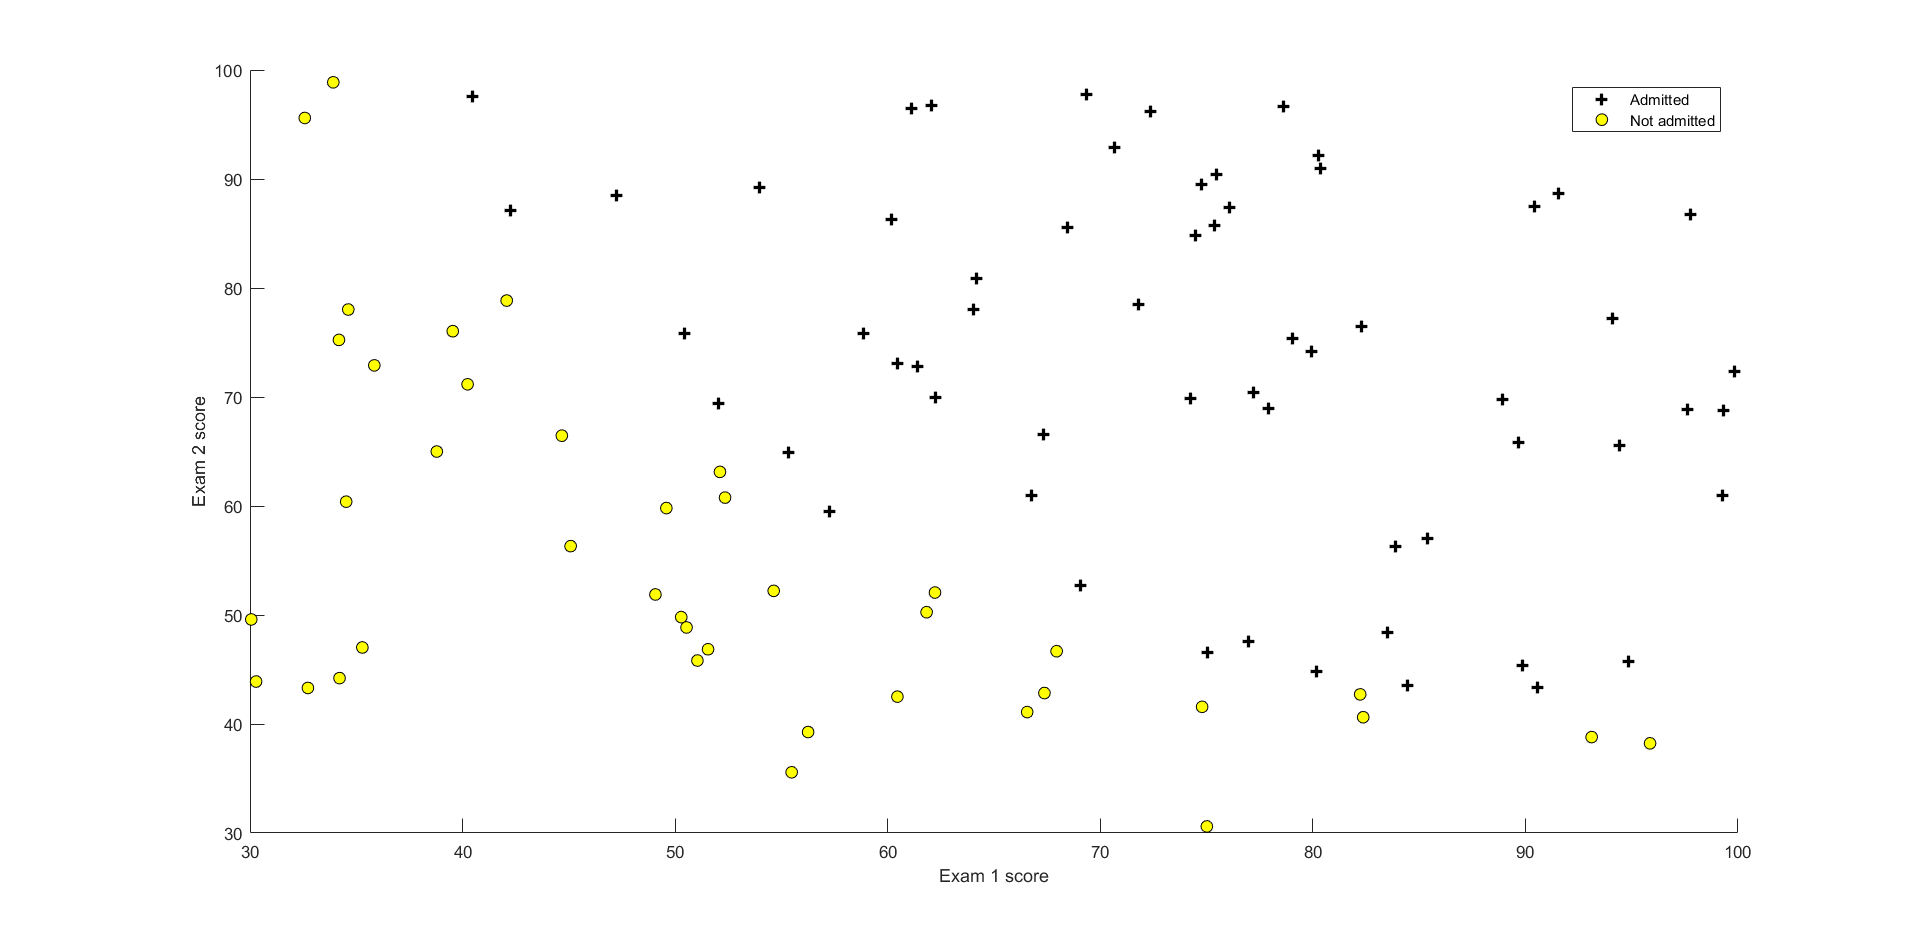
\includegraphics[height=5cm, width=\linewidth]{../exercise2_1/images/ex1_dataset.png}
			\caption{Dataset}
		\end{subfigure}%
		~
		\begin{subfigure}[t]{0.5\textwidth}
			\centering
			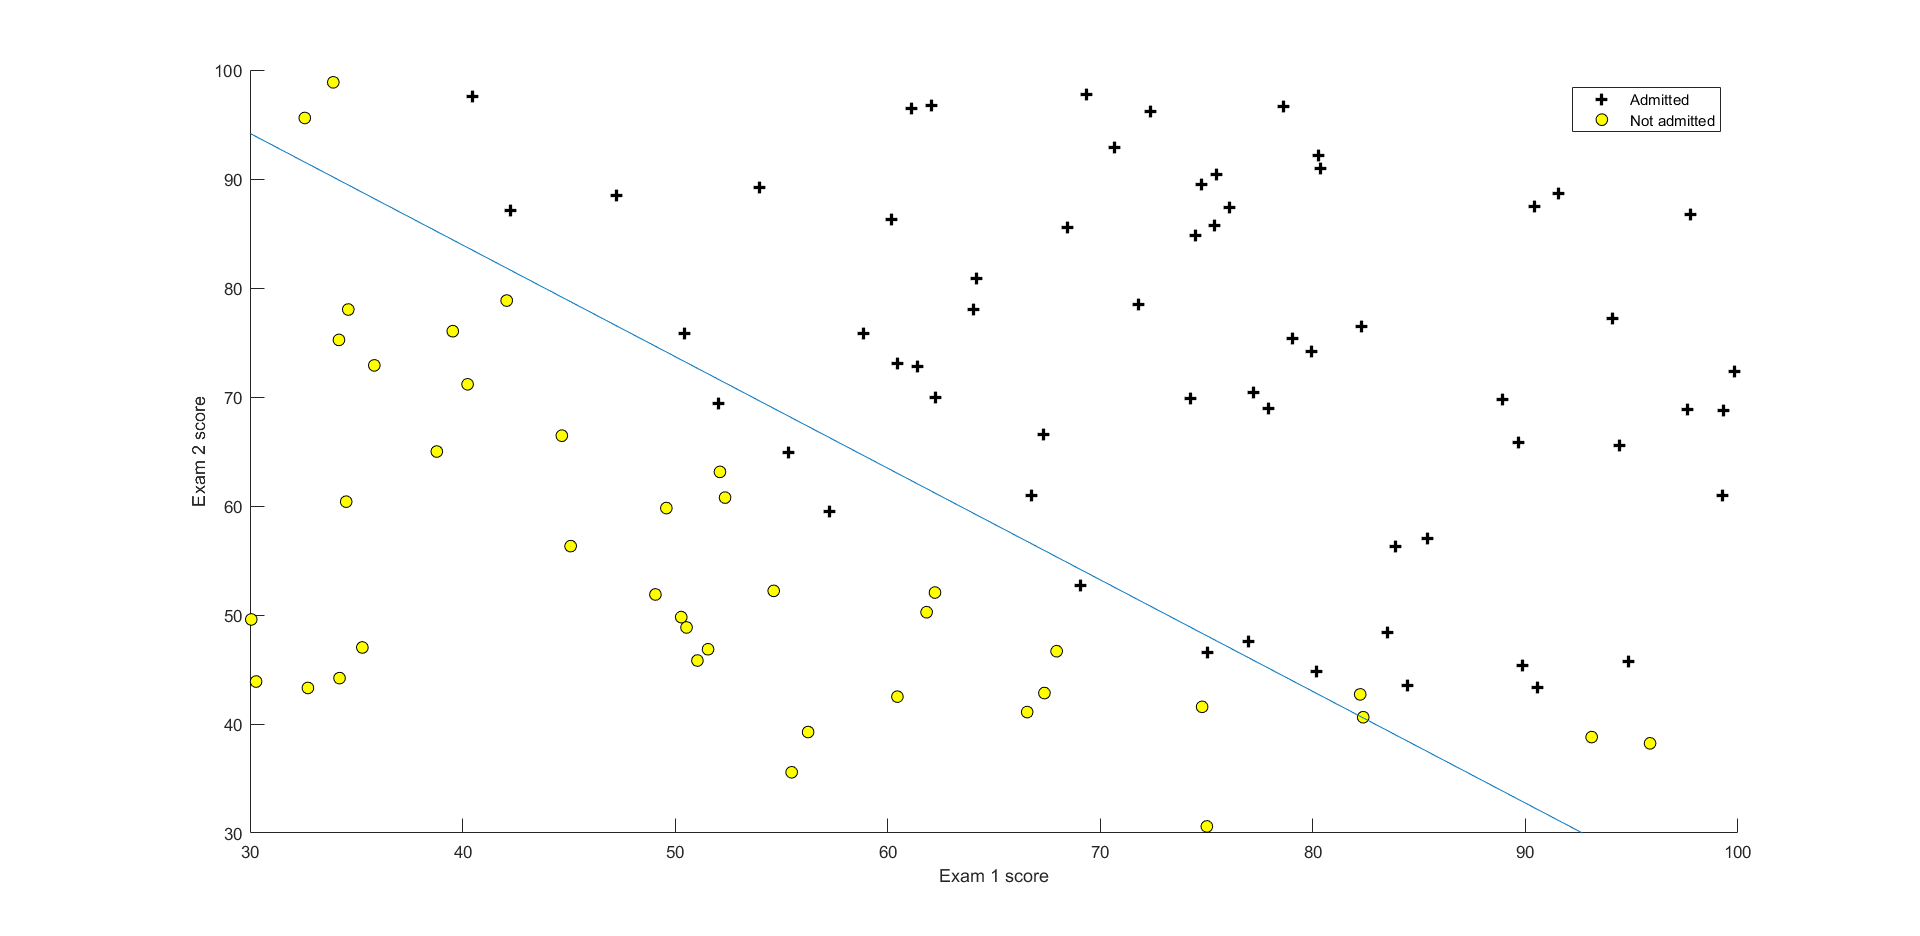
\includegraphics[height=5cm, width=\linewidth]{../exercise2_1/images/ex1_result.png}
			\caption{Results}
		\end{subfigure}
	\end{figure}
	
	
\section*{Άσκηση 2: Λογιστική Παλινδρόμηση με Ομαλοποίηση}
	Στη συγκεκριμένη άσκηση μας ζητήθηκς να εφαρμόσουμε ομαλοποιημένη λογιστική παλινδρόμηση για να προβλέψουμε αν τα μικροτσίπ από μια μονάδα κατασκευής περνούν τον έλεγχο ποιότητας. Κατά τη διάρκεια του ελέγχου ποιότητας, κάθε μικροτσίπ περνάει από διάφορες δοκιμές, για να εξασφαλιστεί ότι λειτουργεί σωστά. \\
	
	\noindent
	Υποθέτουμε ότι υπάρχουν τα αποτελέσματα δύο διαφορετικών δοκιμών για ορισμένα μικροτσίπ. Από αυτά τα αποτελέσματα θα πρέπει να καθορίσουμε αν τα μικροτσίπ θα γίνουν αποδεκτά ή θα απορριφθούν. Θα χρησιμοποιήσουμε δεδομένα	προηγούμενων δοκιμών για να δημιουργήσουμε ένα μοντέλο λογιστικής παλινδρόμησης. \\
	
	\noindent
	Πιο συγκεκριμένα, απεικονίζουμε τα δεδομένα σε ένα χώρο μεγαλύτερης διάστασης όπου τα δεδομένα μπορούν να διαχωριστούν ευκολότερα. Για το σκοπό αυτό δημιουργήθηκε η συνάρτηση mapFeature() η οποία απεικονίζει τα χαρακτηριστικά σε όλους τους όρους πολυωνύμων $x_{1}$ και $x_{2}$ μέχρι και βαθμού 6. Ειδικότερα, η συγκεκριμένη συνάρτηση υλοποιεί την παρακάτω σχέση
	
	\begin{align*}
		P(x_{1},x_{2}) &= \sum_{i=0}^{6} \sum_{j=0}^{i} x^{i-j}_{1} \cdot x^{j}_{2}
	\end{align*}
	
	\noindent
	Επιπλέον, η ομαλοποιημένη συνάρτηση κόστους δίνεται από την σχέση
	\begin{align*}
		J(θ) = \frac{1}{m} \cdot \sum_{i=1}^{m}  \left (-y^{(i)} \cdot \ln(y^{(i)}) - (1-y^{(i)}) \cdot \ln (1 - y^{(i)}) \right) + \frac{λ}{2 m} \cdot \sum_{j=1}^{n} θ_{j}^{2} 
	\end{align*}

	\noindent
	Για να βρούμε το j-στοιχείο της κλίση του σφάλματος εργαζόμαστε όπως και στην άσκηση 1 με μοναδική διαφορά ότι έχουμε να υπολογίσουμε την παρακάτω παράγωγο
	
	\begin{align*}
		\frac{\partial \left(\frac{λ}{2 m} \cdot  \sum_{i=1}^{n} θ_{j}^{2} \right)}{\partial θ_{j}}
		&= \frac{λ}{2 m} \cdot \sum_{i=1}^{n} \frac{\partial \left( θ_{j}^{2} \right)}{\partial θ_{j}} \\
		&= \frac{λ}{2 m} \cdot \sum_{i=1}^{n} 2 \cdot θ_{j} \\
		&= \frac{λ}{2 m} \cdot 2 \cdot \sum_{i=1}^{n}  θ_{j} \\
		&= \frac{λ}{m} \cdot \sum_{i=1}^{n}  θ_{j}
	\end{align*}

	
	\noindent
	Συνεπώς, το j-στοιχείο της κλίσης του σφάλματος είναι
	\begin{align*}
		\frac{\partial J(θ)}{\partial θ_{j}} &= \frac{1}{m} \cdot \sum_{i=1}^{m} \left( h_{θ}(x^{(i)}) - y^{(i)} \right) \cdot x^{(i)}_{j} + \frac{λ}{m} \cdot \sum_{i=1}^{n}  θ_{j}
	\end{align*}
	
	\noindent
	Aρχικά, το dataset πάνω στο οποίο εφαρμόζουμε την μέθοδο της Λογιστικής Παλινδρόμησης με Ομαλοποίηση είναι το εξής
	\begin{figure}[h!]
		\centering
		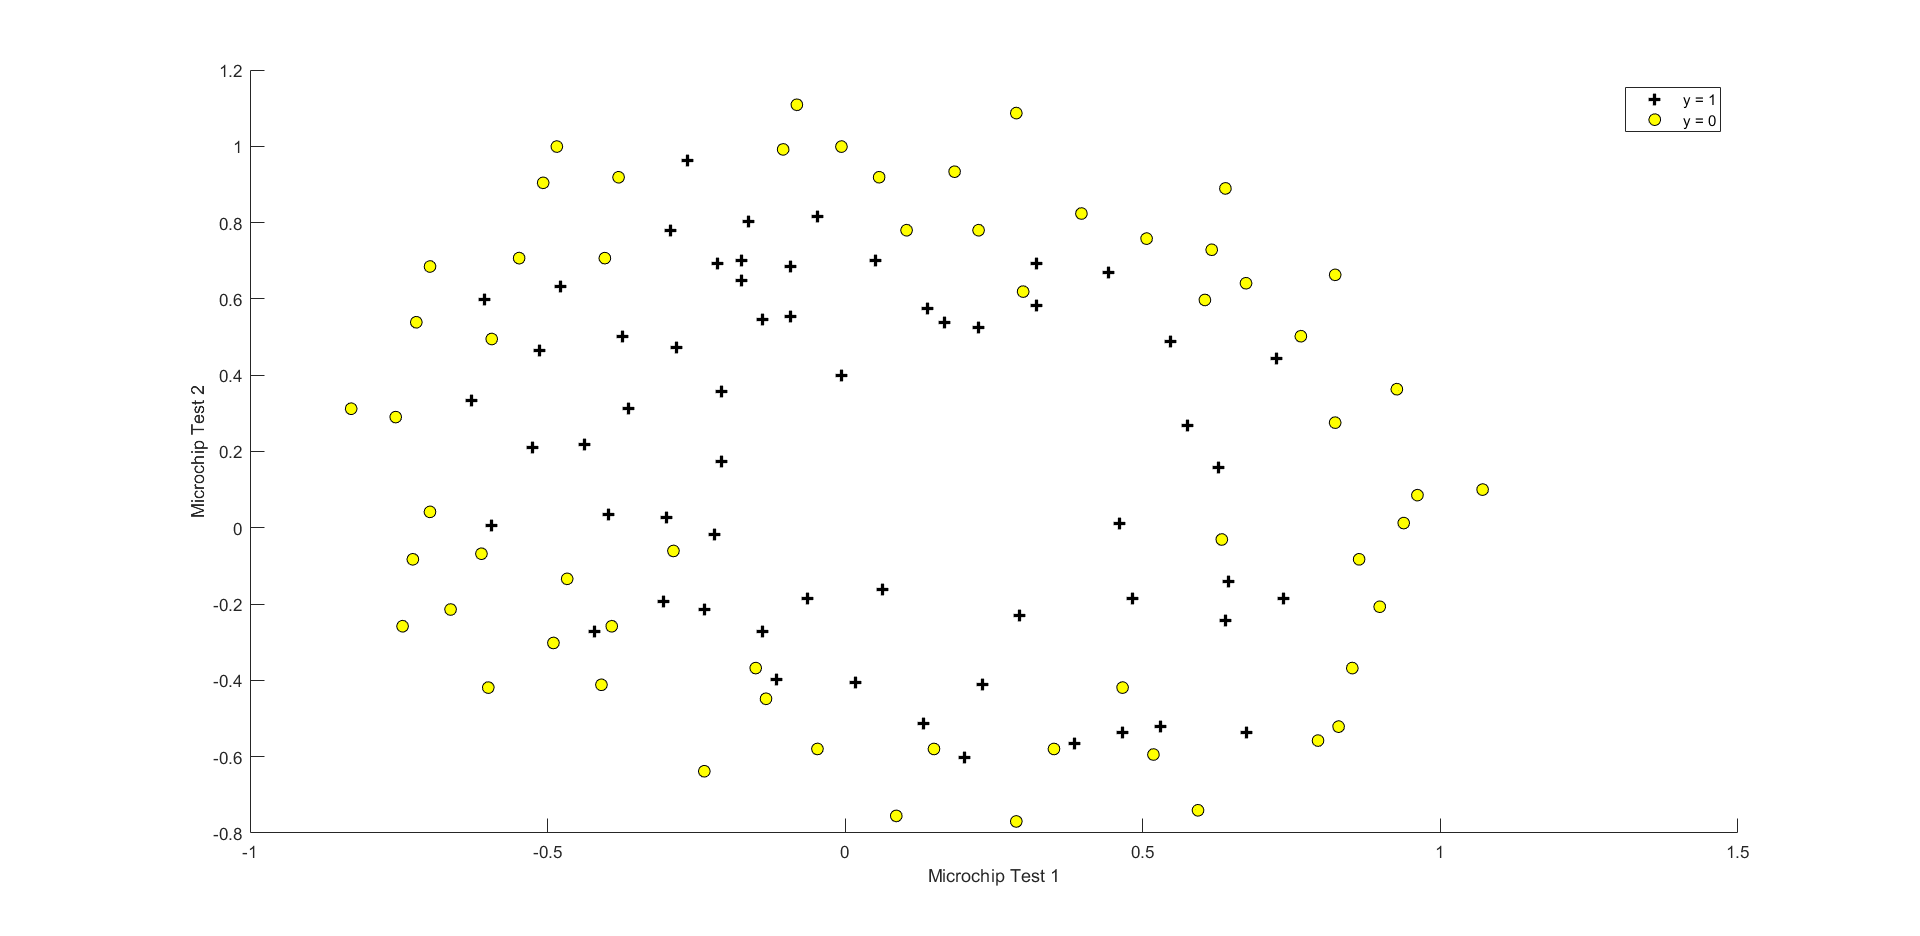
\includegraphics[height=6cm,width=6cm]{../exercise2_2/images/ex2_dataset.png}
		\caption{Dataset}
	\end{figure}

	\noindent
	Για ο σκοπό της συγκεκριμένης άσκησης δημιουργήθηκε μια συνάρτηση sigmoid() και predict() ακριβώς ίδιες με της προηγούμενης άσκησης. Επιπλέον, δημιουργήθηκε και μια συνάρτηση costFunctionReg() στην οποία υπολογίζουμε το κόστος και την κλίση του σφάλματος με βάση τους παραπάνω δύο τύπους.
	
	\pagebreak
	\noindent
	Όσον αφορά τα αποτελέσματα του αλγορίθμου, το κόστος που προκύπτει για λ=1 και θ αρχικοποιημένo στο 0 είναι 0.693147. Παρακάτω παρουσιάζονται τα αποτελέσματα για διαφορετικές τιμές του της παραμέτρου λ.
	\begin{figure}[h!]
		\centering
		\begin{subfigure}[t]{0.5\textwidth}
			\centering
			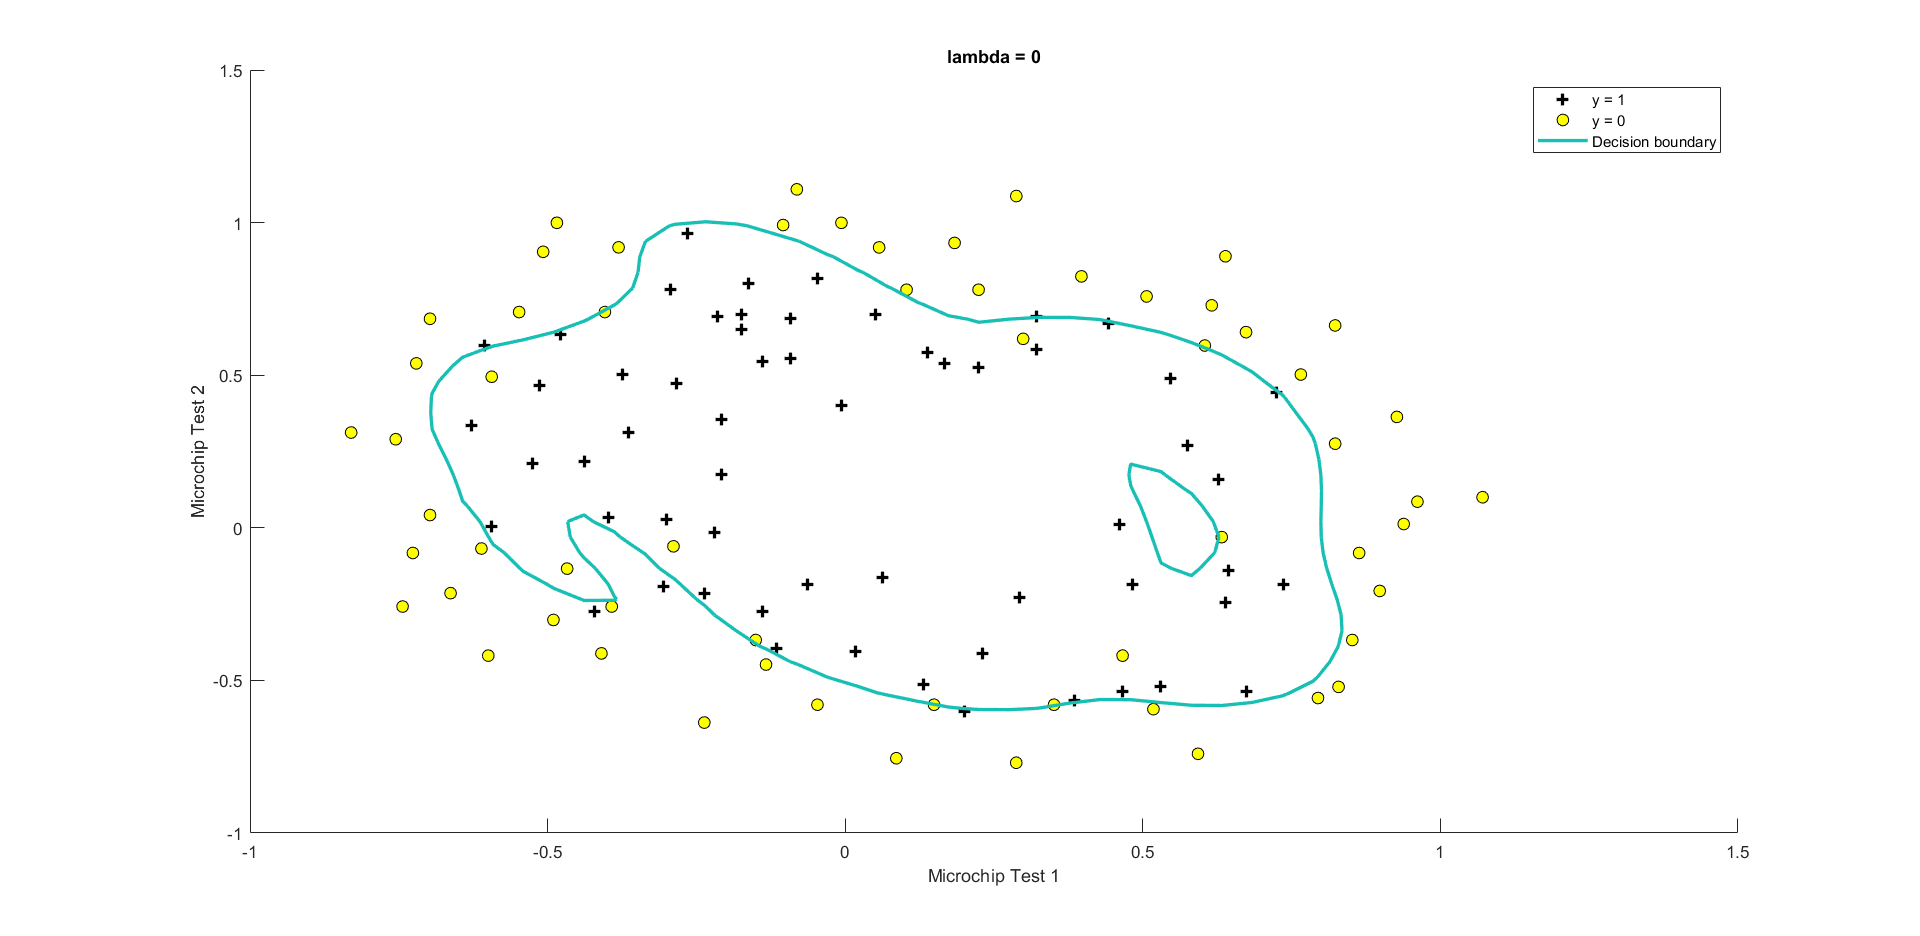
\includegraphics[height=5cm, width=\linewidth]{../exercise2_2/images/ex2_lambda_0.png}
			\caption{λ = 0}
		\end{subfigure}%
		~
		\begin{subfigure}[t]{0.5\textwidth}
			\centering
			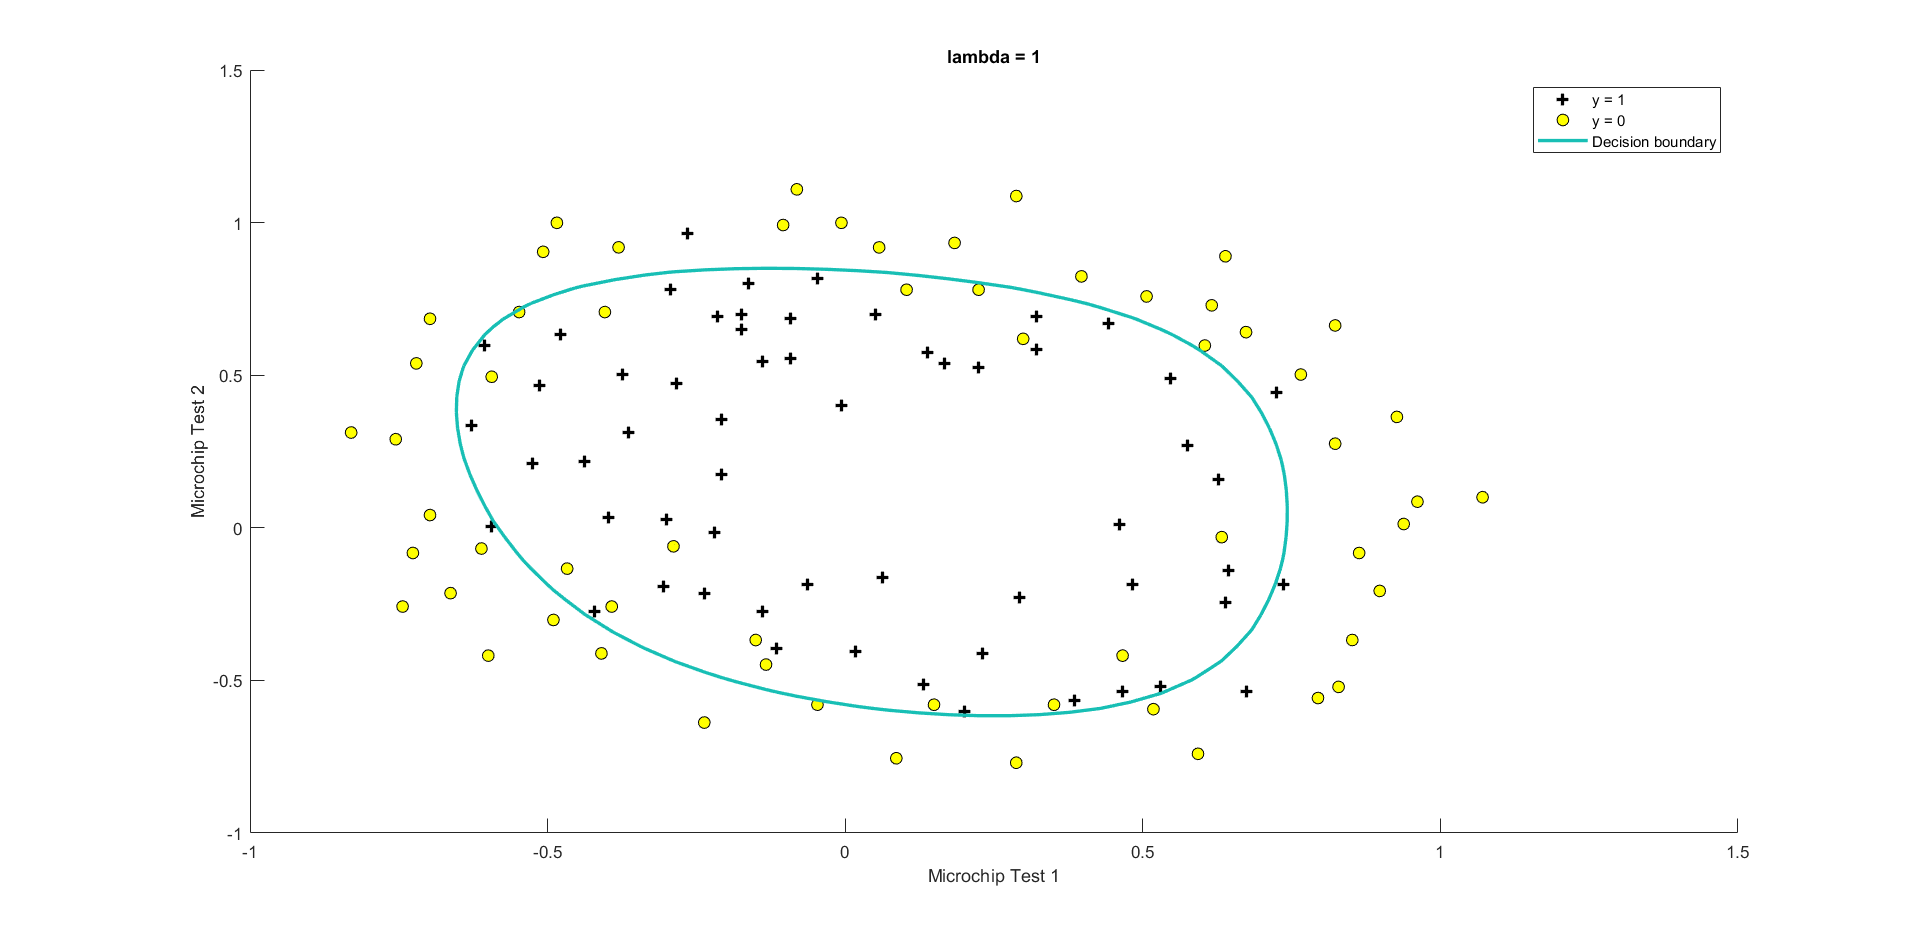
\includegraphics[height=5cm, width=\linewidth]{../exercise2_2/images/ex2_lambda_1.png}
			\caption{λ = 1}
		\end{subfigure}
	
		\begin{subfigure}[t]{0.5\textwidth}
			\centering
			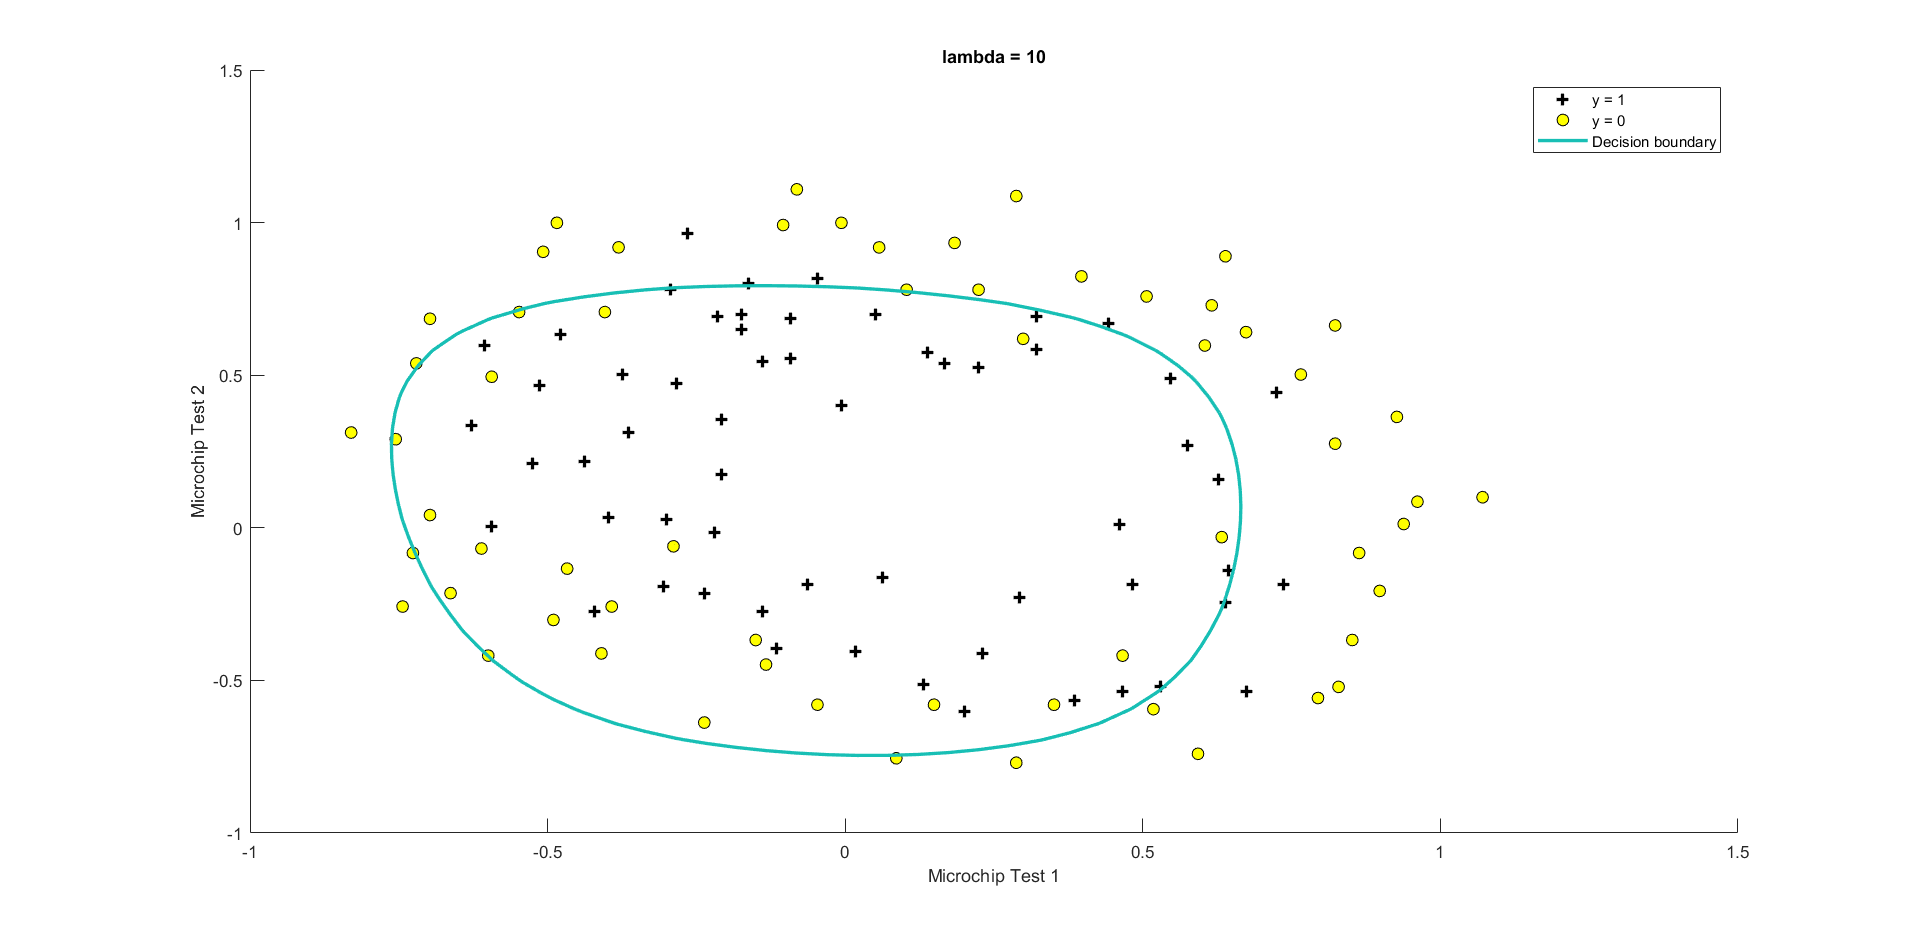
\includegraphics[height=5cm, width=\linewidth]{../exercise2_2/images/ex2_lambda_10.png}
			\caption{λ = 10}
		\end{subfigure}%
		~
		\begin{subfigure}[t]{0.5\textwidth}
			\centering
			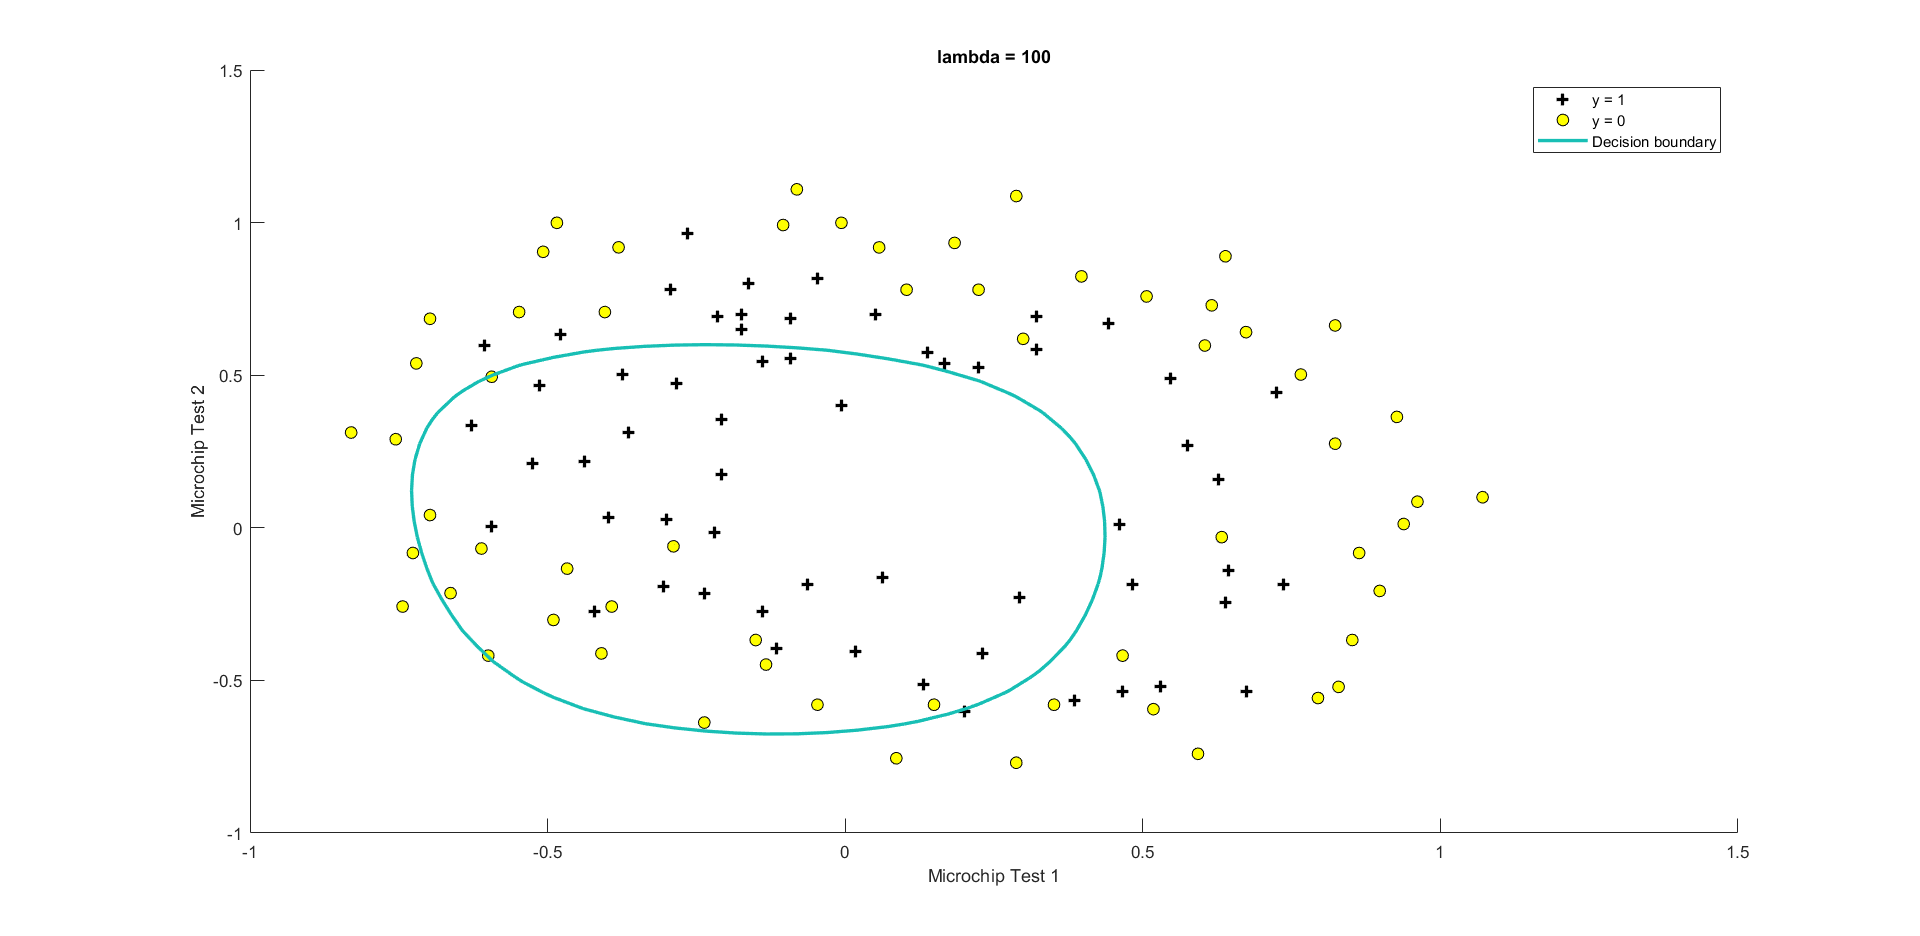
\includegraphics[height=5cm, width=\linewidth]{../exercise2_2/images/ex2_lambda_100.png}
			\caption{λ = 100}
		\end{subfigure}
	\end{figure}
	
	\begin{table}[!ht]  
		\centering
		\begin{tabular}{|c|c|c|c|c|}
			\cline{2-5}
			\multicolumn{1}{c|}{} & λ=0 & λ=1 & λ=10  & λ=100\\ \hline
			Κόστος J & 0.2226  & 0.5290   & 0.6482 & 0.6865  \\ \hline
			Train Accuracy & 88.135593 & 83.050847   & 74.576271 & 61.016949 \\ \hline
		\end{tabular}
	\end{table}
	
	\noindent
	Oπως φαίνεται στο παραπάνω πινακάκι και σε συνδυασμό με τα αποτελέσματα των γραφικών παρατηρούμε ότι όσο αυξάνεται η τιμή της παραμέτρου λ, τόσο μειώνεται το Train Accuracy, ενώ το decision boundary γίνεται όλο και πιο μικρό με αποτέλεσμα να γίνονται περισσότερα σφάλματα κατα την εκπαίδευση. Τέλος, όσον αφορά το κόστος βλέπουμε ότι αυξάνεται, γεγονός που είναι λογικό με βάση και τις προηγούμενες παρατηρησεις.
	
\section*{Άσκηση 3: Εκτίμηση Παραμέτρων (Maximum Likelihood)}
	Έστω n δείγματα D = $\{x_{1}, x_{2}, \cdots, x_{n},\}$ παράγονται ανεξάρτητα από μια κατανομή Poisson με παράμετρο λ, όπου η PDF δίνεται από την παρακάτω σχέση
	
	\begin{align*}
		p(x|λ) &= \frac{λ^{x} \cdot e^{-λ}}{x!}, \tab x = 0, 1, 2, \cdots , \tab λ > 0
	\end{align*}
	
	\pagebreak
	\noindent
	Aρχικά, η συνάρτηση likelihood για την κατανομή Poisson δίνεται από τη σχέση:
	
	\begin{align*}
		L(λ|x_{1},x_{1}, \cdots, x_{n}) &= \prod_{i=1}^{n} p(x|λ)  = \prod_{i=1}^{n} \frac{λ^{x_{i}} \cdot e^{-λ}}{x_{i}!}
	\end{align*}

	\noindent
	Επειδή ο λογάριθμος είναι γνησίως μονότονη (αύξουσα) συνάρτηση, η παράμετρος λ που μεγιστοποιεί τον λογάριθμο της πιθανοφάνειας(log-likelihood), θα μεγιστοποιεί και την πιθανοφάνεια. Συνεπώς, ορίζουμε το log-likelihood ως εξής:
	
	\begin{align*}
		\mathcal{L}(λ|x_{1},x_{2}, \cdots, x_{n}) &= \ln \left( \prod_{i=1}^{n} \frac{λ^{x_{i}} \cdot e^{-λ}}{x_{i}!}\right) \\
												  &= \sum_{i=1}^{n} \ln \left( \frac{λ^{x_{i}} \cdot e^{-λ}}{x_{i}!}\right) \\
												  &= \sum_{i=1}^{n} [\ln(e^{-λ}) + \ln(λ^{x_{i}}) - \ln(x_{i}!)] \\
												  &= \sum_{i=1}^{n} [-λ + x_{i} \cdot \ln(λ) - \ln(x_{i}!)] \\
												  &= \sum_{i=1}^{n} -λ + \sum_{i=1}^{n} x_{i} \cdot \ln(λ) - \sum_{i=1}^{n} \ln(x_{i}!) \\
												  &= -λ \cdot n + \ln(λ) \cdot \sum_{i=1}^{n} x_{i}   - \sum_{i=1}^{n} \ln(x_{i}!)
	\end{align*}
	
	\noindent
	Aν παραγωγίσουμε την παραπάνω log-likelihood ως προς λ και θέσουμε την παράγωγο ίση με 0 έχουμε:
	\begin{align*}
		\frac{\partial \mathcal{L}(λ|x_{1},x_{2}, \cdots, x_{n})}{\partial λ} &= 0 \Rightarrow \\
		\frac{\partial (-λ \cdot n + \ln(λ) \cdot \sum_{i=1}^{n} x_{i} - \sum_{i=1}^{n} \ln(x_{i}!))}{\partial λ} &= 0 \Rightarrow \\
		\frac{\partial (-λ \cdot n)}{\partial λ} + 
		\frac{\partial (\ln(λ) \cdot \sum_{i=1}^{n} x_{i})}{\partial λ} - 
		\frac{\partial (\sum_{i=1}^{n} \ln(x_{i}!))}{\partial λ} &= 0 \Rightarrow \\
		-n + \frac{1}{λ} \cdot \sum_{i=1}^{n} x_{i} - 0 &= 0 \Rightarrow \\
		\frac{1}{λ} \cdot \sum_{i=1}^{n} x_{i} &= n \Rightarrow \\
		λ &=\frac{1}{n} \cdot \sum_{i=1}^{n} x_{i}	 
	\end{align*}
	
	\noindent
	Συνεπώς, παρατηρούμε ότι ο maximum likelihood εκτημητής είναι απλώς ο δειγματικός μέσος των n παρατηρήσεων μεσα στο δειγματικό χώρο. Αυτό το αποτέλεσμα είναι διασιθητικά σωστό καθώς η αναμενόμενη τιμή μιας Poisson τυχαίας μεταβλητής είναι ίση με την παράμετρο λ και ο δειγματικός μέσος είναι ένας σωστός εκτιμητής της αναμενόμενης τιμής.
	
\section*{Άσκηση 4: Εκτίμηση Παραμέτρων και Ταξινόμηση (ΜL - Naïve Bayes Classifier)}	
	Στη συγκεκριμένη άσκηση μας ζητήθηκε να υλοποιήσουμε έναν Naive ταξινομητή Bayes για την αναγνώριση των ψηφίων που υπάρχουν στη βάση δεδομένων 'digits.mat'. Στη συγκεκριμένη βάση υπάρχουν ψηφία από το 0 ως το 9 τα οποία είναι αποθηκευμένα ως μια ασπρόμαυρη εικόνα με διαστάσεις 28 $\times$ 28 που μπορεί να αναπαρασταθεί ως ένα διάνυσμα 784 $\times$ 1. Eπιπλέον, υπάρχουν δείγματα για εκπαίδευση και δείγματα δοκιμής. \\
	
	Αρχικά, οπτικοποιούμε το 43ο ψηφίο της κλάσης 7. Παρακάτω φαίνεται η εικόνα του ψηφίου.
	
	 \begin{figure}[h!]
	 	\centering
	 	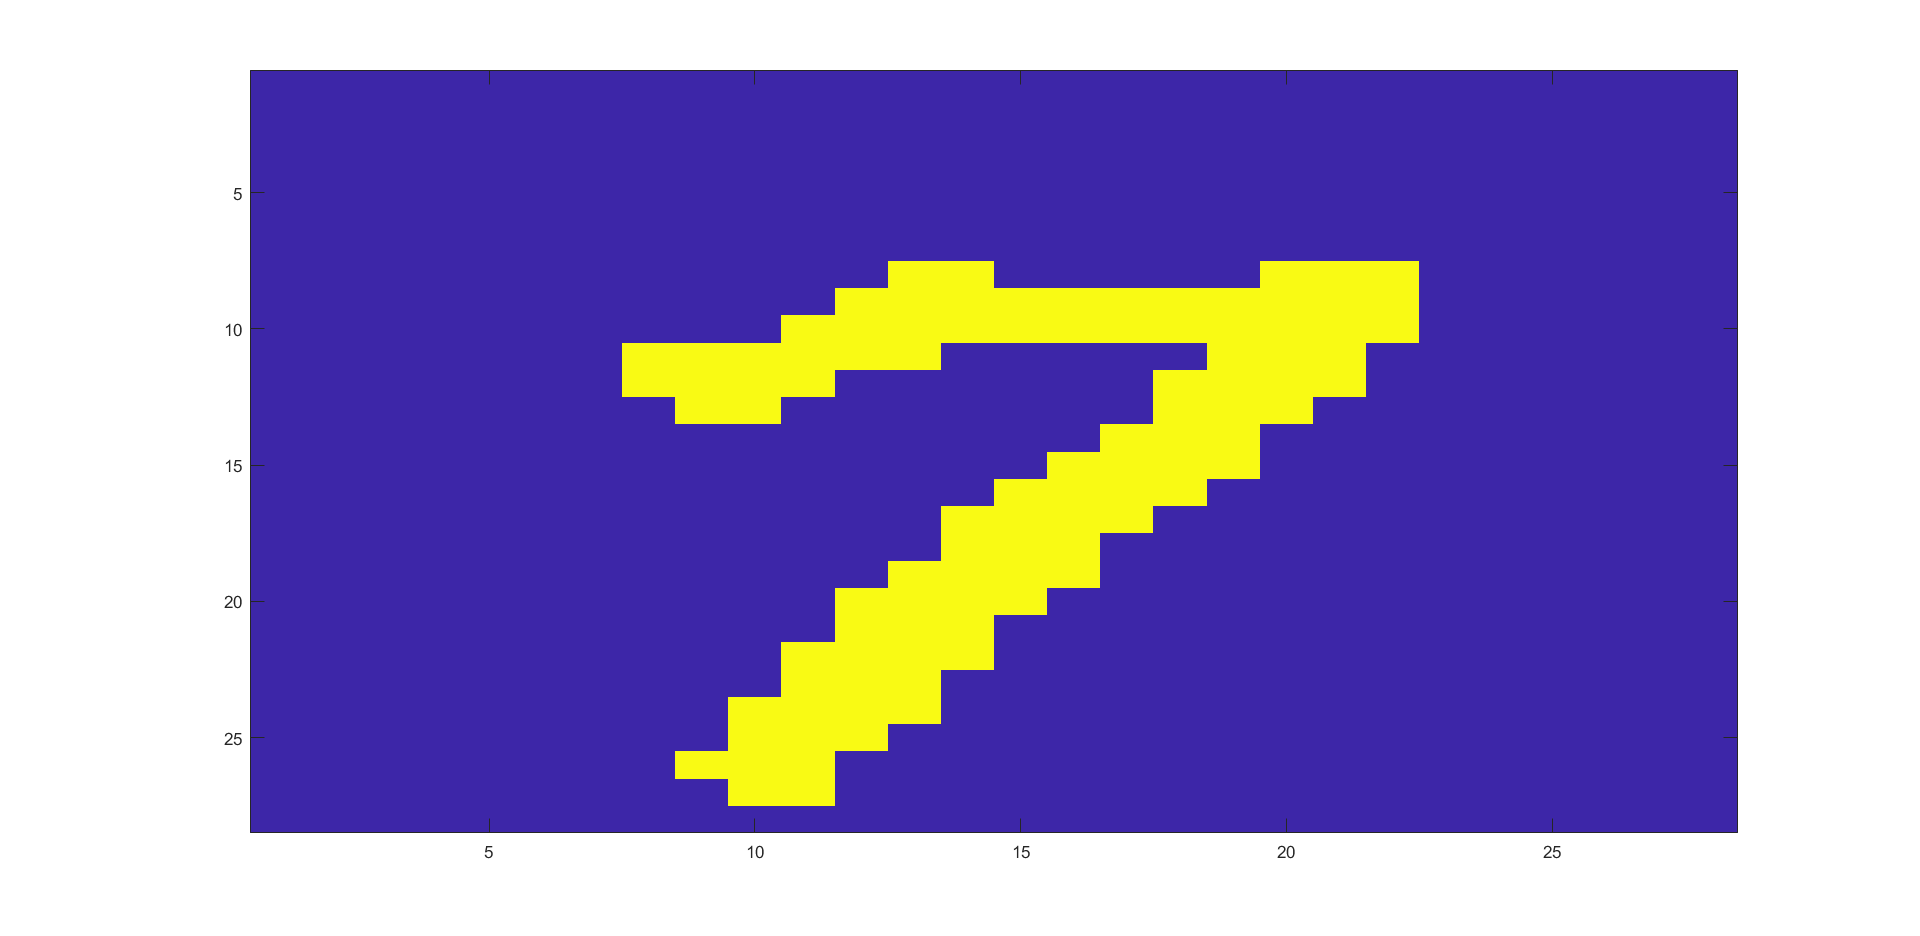
\includegraphics[height=6cm,width=6cm]{../exercise2_4/images/ex4_digit_7.png}
	 	\caption{Digit 7}
	 \end{figure}
	
	\noindent
	Έστω ότι στον naive Bayes ταξινομητή τα χαρακτηριστικά, τα οποία στην περίπτωσή μας, είναι τα pixel των εικόνων, είναι ανεξάρτητα και ότι ακολουθούν κατανομή Bernoulli με PDF η οποία δίνεται από τη σχέση
	
	\begin{align*}
		p(x) &= p^{x} \cdot (1-p)^{1-x}
	\end{align*}
	
	\noindent
	Η συνάρτηση likelihood για την κατανομή Βernoulli δίνεται από τη σχέση:
	
	\begin{align*}
		L(p|x_{1}, x_{2}, \cdots, x_{n}) &= \prod_{i=1}^{n} p(x)  = \prod_{i=1}^{n} p^{x_{i}} \cdot (1-p)^{1-x_{i}}
	\end{align*}

	\noindent
	Επειδή ο λογάριθμος είναι γνησίως μονότονη (αύξουσα) συνάρτηση, η παράμετρος λ που μεγιστοποιεί τον λογάριθμο της πιθανοφάνειας(log-likelihood), θα μεγιστοποιεί και την πιθανοφάνεια. Συνεπώς, ορίζουμε το log-likelihood ως εξής:
	
	\begin{align*}
		\mathcal{L}(p|x_{1},x_{2}, \cdots, x_{n}) &= \log \left( \prod_{i=1}^{n} p^{x_{i}} \cdot (1-p)^{1-x_{i}} \right) \\
		&= \sum_{i=1}^{n} \log \left( p^{x_{i}} \cdot (1-p)^{1-x_{i}} \right) \\
		&= \sum_{i=1}^{n} \left[ \log ( p^{x_{i}} ) + \left( \log (1-p)^{1-x_{i}} \right) \right] \\
		&= \sum_{i=1}^{n} \left( x_{i} \cdot \log (p) + (1-x_{i}) \cdot \log (1-p) \right) \\
		&= \log (p) \cdot \sum_{i=1}^{n} x_{i} + \log (1-p) \cdot \sum_{i=1}^{n} (1-x_{i})
	\end{align*}

	\pagebreak
	\noindent
	Aν παραγωγίσουμε την παραπάνω log-likelihood ως προς λ και θέσουμε την παράγωγο ίση με 0 έχουμε:
	\begin{align*}
		\frac{\partial \mathcal{L}(p|x_{1},x_{2}, \cdots, x_{n})}{\partial p} &= 0 \Rightarrow \\
		\frac{\partial (\log (p) \cdot \sum_{i=1}^{n} x_{i} + \log (1-p) \cdot \sum_{i=1}^{n} (1-x_{i}))}{\partial p} &= 0 \Rightarrow \\
		\frac{\partial (\log (p) \cdot \sum_{i=1}^{n} x_{i})}{\partial p} + 
		\frac{\partial (\log (1-p) \cdot \sum_{i=1}^{n} (1-x_{i}))}{\partial p} &= 0 \Rightarrow \\	
		\frac{1}{p} \cdot \sum_{i=1}^{n} x_{i} - \frac{1}{1 - p} \cdot \sum_{i=1}^{n} (1-x_{i}) &= 0 \Rightarrow \\	
		\frac{1}{1 - p} \cdot \sum_{i=1}^{n} (1-x_{i}) & = \frac{1}{p} \cdot \sum_{i=1}^{n} x_{i} \Rightarrow \\		
		\frac{n}{1 - p}  - \frac{1}{1 - p} \cdot \sum_{i=1}^{n} x_{i} &= \frac{1}{p} \cdot \sum_{i=1}^{n} x_{i} \Rightarrow \\
		n \cdot p  - p \cdot \sum_{i=1}^{n} x_{i} &= (1 - p) \cdot \sum_{i=1}^{n} x_{i} \Rightarrow \\
		n \cdot p  - p \cdot \sum_{i=1}^{n} x_{i} &= \sum_{i=1}^{n} x_{i} - p \cdot \sum_{i=1}^{n} x_{i } \Rightarrow \\
		n \cdot p &= \sum_{i=1}^{n} x_{i} \Rightarrow \\
		p &= \frac{1}{n} \cdot \sum_{i=1}^{n} x_{i}
	\end{align*}

	\noindent
	Aρχικά, όσον αφορά την υλοποίηση έπρεπε να υπολογίσουμε το $p^{y_{i}}$ της κάθε κλάσης με βάση τον παραπάνω τύπο που υπολογίστηκε προηγουμένως, δηλαδή αθροίζουμε όλες τις γραμμές της κάθε κλάσης και διαιρούμε με το συνολικό πλήθος εικόνων της κάθε κλάσης που είναι 500.
	
	\noindent
	Στη συνέχεια, για την εκπαίδευση για κάθε κλάση και για κάθε εικόνα της κάθε κλάσης υπολογίζουμε τη log-likelihood. Ωστόσο, πριν από αυτό το βήμα επειδή κάποιες πιθανότητες έβγαιναν 0, αντικαταστήσαμε όλα τα μηδενικά του πίνακα με τις πιθανότητες με την τιμή 0.0000001, για να μπορεί να υπολογιστεί ο λογάριθος χωρίς κάποιο πρόβλημα. Επιπλέον, μόλις υπολογίσουμε και αποθηκεύσουμε όλες τις 500 log-likelihood μιας κλάσης πολλαπλασιάζουμε το ανάστροφο των εικόνων train με τον πίνακα όπου έχουμε αποθηκεύουμε τις likelihoods έτσι, ώστε να προκύψει η εκπαιδευμένη εικόνα της κάθε κλάσης. Τα αποτελέσματα φαίνονται παρακάτω
	
	\begin{figure}[h!]
		\centering
		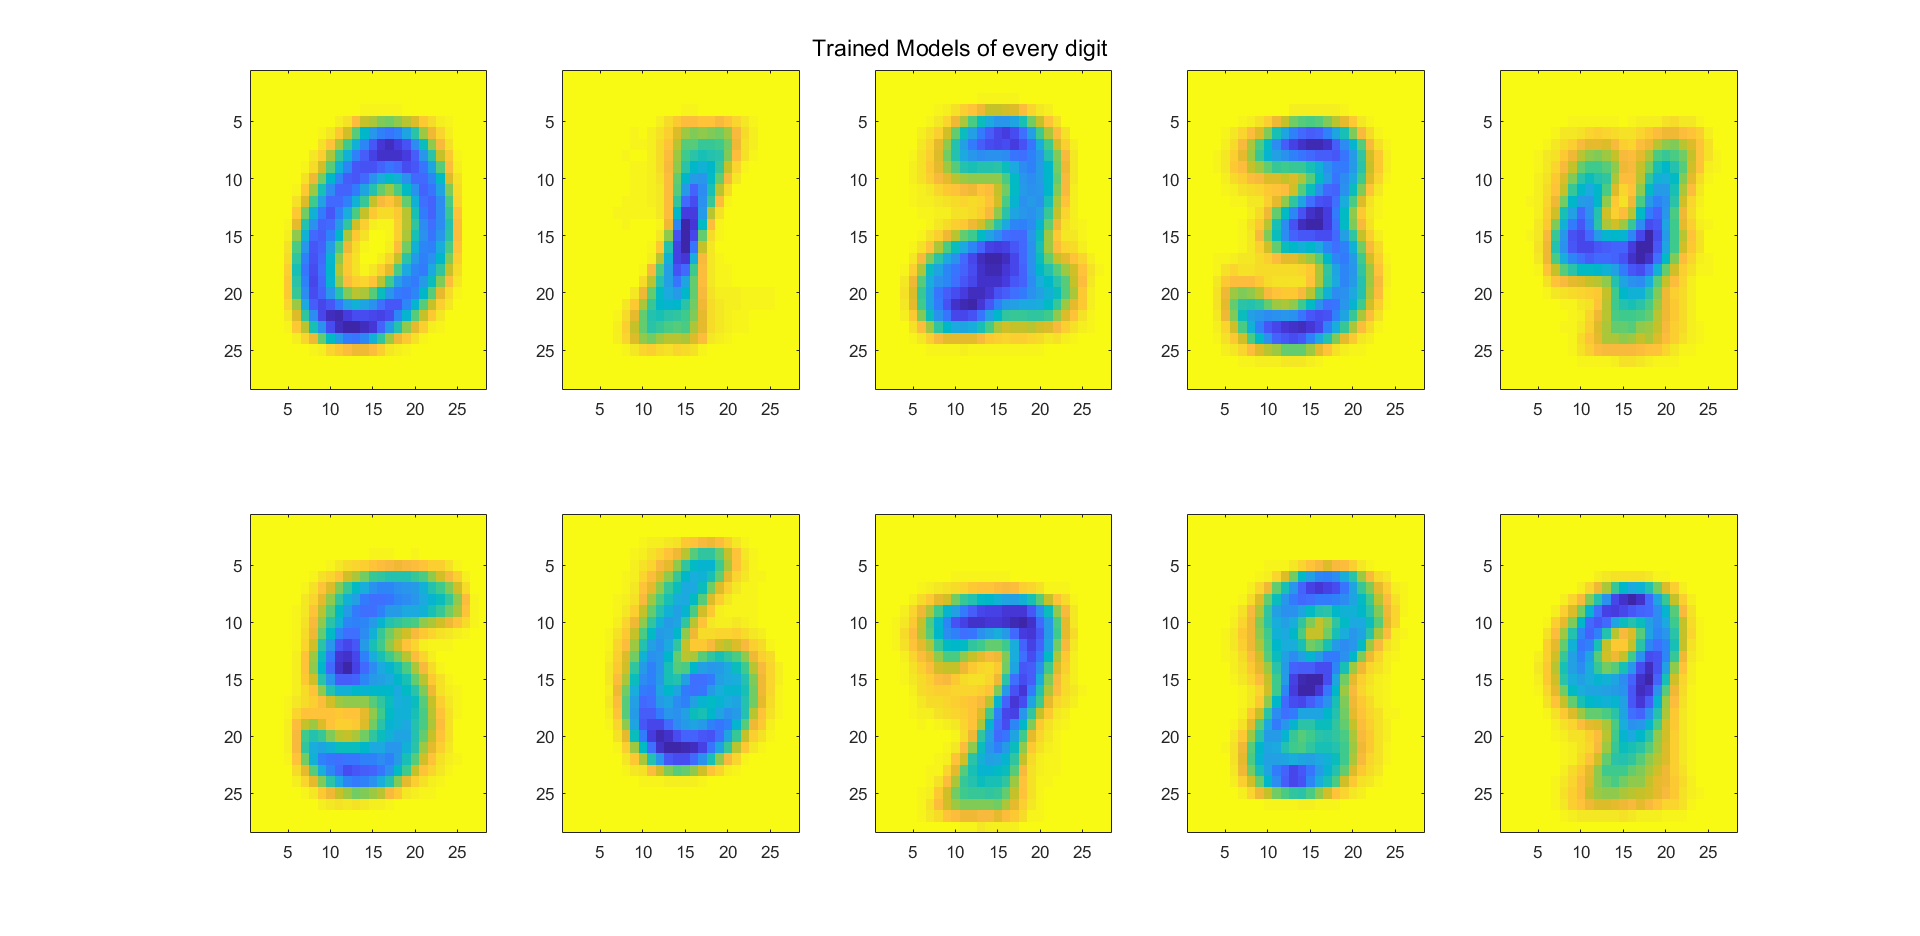
\includegraphics[height=6cm,width=\linewidth]{../exercise2_4/images/ex4_trained_model.png}
	\end{figure}
	
	\pagebreak
	\noindent
	Για τη δοκιμή του Naive Bayes Classifier χρησιμοποιήθηκαν οι εικόνες δοκιμής του 'digit.mat'. Eιδικότερα, όπως και στον προηγούμενο υπολογισμό, για κάθε κλάση και για κάθε εικόνα μέσα στην κάθε κλάση υπολογίζουμε τις 10 πιθανότητες likelihood και βρίσκουμε την εικόνα με τη μέγιστη τιμή likelihood. \\
	
	\noindent
	Για τον υπολογισμό του accuracy για το κάθε ψηφίο και το συνολικό accuracy, έχουμε 2 counters τους οποίους αυξάνουμε μόνο όταν το index, το οποίο δείχνει παράλληλα και την κλάση i, είναι ίσο με το index του array που επιστρέφει η συνάρτηση max() της matlab. Η μοναδική διαφορά μεταξύ των counter είναι ότι τον πρώτο κάθε φορά που αλλάζουμε κλάση τον αρχικοποιούμε στο 0.\\ 
	
	\noindent
	Tέλος, όσον αφορά το confusion matrix αυτός υπολογίζεται ως εξής: Συμπληρώνεται ανά γραμμή και κάθε φορά αυξάνουμε το κελί (i,j) όπου i είναι η κλάσηγραμμή που βρισκόμαστε και το j είναι το index που μας επιστρέφει η συνάρτηση max().\\
	
	\noindent
	\underline{Confussion Matrix}\\
	\begin{table}[h!]
		\centering 
		\begin{tabular}{|c|c|c|c|c|c|c|c|c|c|} 
			\hline
			0,882 & 0 & 0,002 & 0 & 0,004 & 0,06 & 0,026 & 0 & 0,024 & 0,002 \\ \hline
			0 & 0,944 & 0,004 & 0,006 & 0 &	0,026 & 0,008 & 0 & 0,012 & 0 \\ \hline
			0,016 &	0,024 & 0,75 & 0,074 & 0,014 & 0,004& 0,018 & 0,026 & 0,066 & 0,008 \\ \hline
			0,002 &	0,02 & 0,008 & 0,832 & 0,01 & 0,046 & 0,01 & 0,026 & 0,002 & 0,026  \\ \hline
			0,002 & 0,002 & 0,01 & 0 & 0,748 & 0,008 & 0,03 & 0,004 & 0,01 & 0,186 \\ \hline
			0,028 & 0,004 & 0,006 &	0,134 &	0,04 & 0,69 & 0,014 & 0,012 & 0,03 & 0,042\\ \hline
			0,014 &	0,02 & 0,056 & 0 & 0,014 & 0,066 & 0,824 & 0 & 0,006 & 0\\ \hline
			0,002 &	0,042 &	0,018 &	0,006 &	0,03 & 0 & 0 & 0,79 & 0,02 & 0,092\\ \hline
			0,012 &	0,032 &	0,024 & 0,098 &	0,022 & 0,036 & 0,002 & 0,006 & 0,698 & 0,07\\ \hline
			0,006 &	0,016 &	0,006 & 0,016 &	0,102 &	0,014 &	0 & 0,012 & 0,01 & 0,818\\ \hline
		\end{tabular}
	\end{table}

	\noindent
	Πεαρακάτω παρουσιάζεται το accuracy του ταξινομητή για κάθε ψηφίο
	
	\begin{table}[!ht]  
		\centering
		\begin{tabular}{|c|c|c|c|c|c|c|c|c|c|c|}
			\multicolumn{11}{c}{Digits}\\
			\cline{2-11}
			\multicolumn{1}{c|}{} &  0 &  1 &  2  &  3 &  4 &  5 &  6 &  7  &  8 &  9\\ \hline
			Accuracy & 0.882  & 0,944 & 0.75 & 0.832 & 0.748 & 0.69 & 0.824 & 0.79 & 0.698 & 0.818\\ \hline
		\end{tabular}
	\end{table}

	\noindent
	Τέλος, όσον αφορά το συνολικό accuracy του Naive Bayesian Classifier αυτό υπολογίστηκε περίπου 0.7976 ή 79.76 \%.
	
\section*{Άσκηση 5: Support Vector Machines (Αναλυτική βελτιστοποίηση με ΚΚΤ)}
	Έστω δύο κλάσεις $ω_{1}$ και $ω_{2}$ με τα εξής δείγματα η κάθε μία:
	\begin{align*}
		ω_{1}: x^{+} = \{ [3,1]^{T}, [3,-1]^{T}, [5,1]^{T}, [5,-1]^{T} \} \\
		ω_{2}: x^{-} = \{ [1,0]^{T}, [0,1]^{T}, [0,-1]^{T}, [-1,0]^{T} \}
	\end{align*}
	\noindent
	Θα χρησιμοποιήσουμε Support Vector Machines (SVM) για να ταξινομήσουμε τις παραπάνω δύο κλάσεις σε δύο διαφορετικές κατηγορίες.\\
	
	\pagebreak
	\begin{figure}[h!]
		\centering
		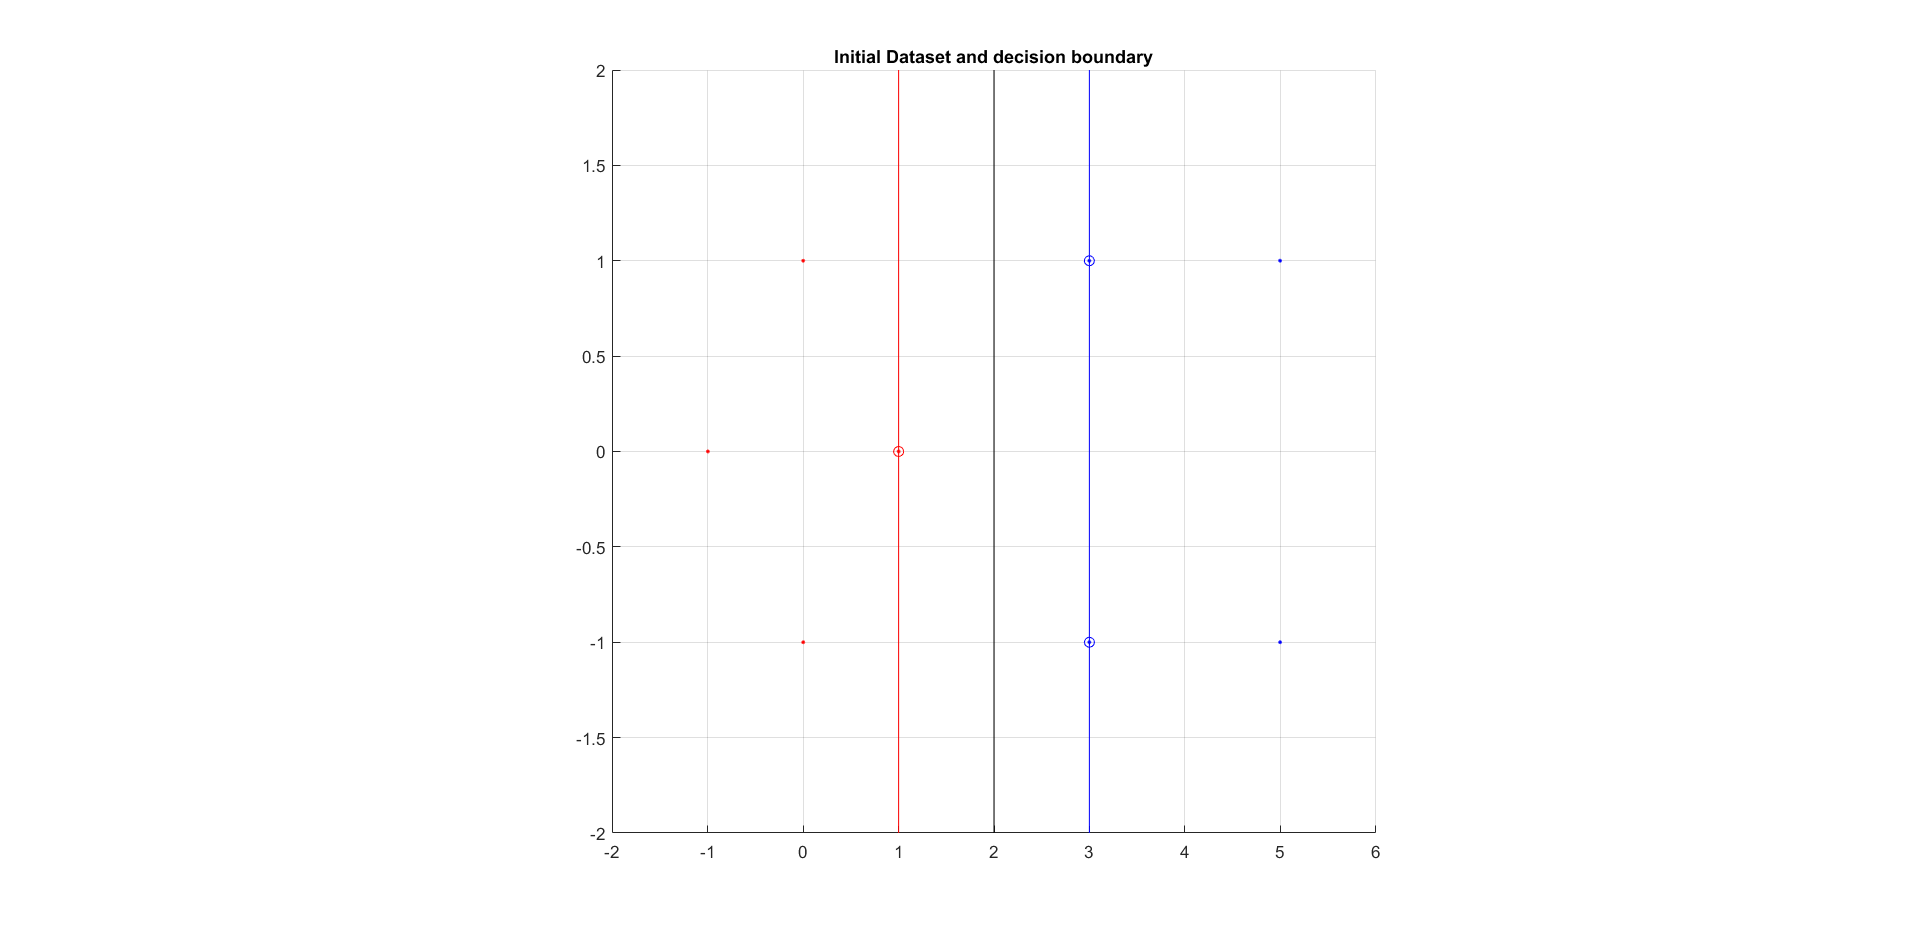
\includegraphics[height=6cm,width=\linewidth]{../exercise2_5/images/ex5_linear.png}
		\caption{Linear SVM}
	\end{figure}
	\noindent
	Με βάση το παραπάνω διάγραμμα απεικόνισης το δειγμάτων, τα support vectors είναι τα εξής:
	\begin{align*}
		S_{1} = [3,1]^{T}, \tab S_{2} = [3,-1]^{T}, \tab S_{3} = [1,0]^{T}
	\end{align*}
	
	\noindent
	Επιπλέον, βλέπουμε ότι η βέλτιστη γραμμή διαχωρισμού των δύο κλάσεων είναι η $x=2$, καθώς σε αυτή την περίπτωση έχουμε το μέγιστο κενό ανάμεσα στις δύο κλάσεις $ω_{1}$ και $ω_{2}$. \\
	
	\noindent
	Για τον αναλυτικό υπολογισμό της εξίσωσης διαχωρισμού θα χρησιμοποιήσουμε πολλαπλασιαστές Lagrange και τις συνθήκες Karush-Khun-Tucker (KKT).\\
	
	\noindent
	Αρχικά, η objective function που θέλουμε να ελαχιστοποιήσουμε είναι η εξής: 
	\begin{align*}
		J(w,b) = \frac{1}{2} \cdot \norm{w}^{2} =  \frac{1}{2} \cdot (w_{1}^{2} + w_{2}^{2})
	\end{align*}
	\noindent
	Οι πειορισμοί κάτω από τους οποίους θα ελαχιστοποιήσουμε την παραπάνω συνάρτηση είναι
	\begin{align*}
		w^{T} \cdot x^{+} + b \ge 1, \forall x^{+} \in ω_{1} \\
		w^{T} \cdot x^{-} + b \le 1, \forall x^{-} \in ω_{2}
	\end{align*}	

	\noindent
	Επιπλέον, έχουμε την παρακάτω σχέση
	\begin{align*}
		\mathcal{L}(w,b,λ) = J(w,w_{0}) - \sum_{i=1}^{N} λ_{i} \cdot [y_{i} \cdot (w^{T} \cdot x^{+} + b) - 1]
	\end{align*}
	
	\noindent 
	Επειδή γνωρίζουμε ότι το offset της γραμμής διαχωρισμού είναι 2 και με σκοπό να περιορίσουμε το χώρο αναζήτησης, θα επιλέξουμε τιμή της παραμέτρου b ίση με -2.
	\begin{align*}
		S_{1} &= [3,1]^{T} : \ \ \ 1 \cdot ( 3 \cdot w_{1} + 1 \cdot w_{2} - 2) \ge 1 \Rightarrow 
								   3 \cdot w_{1} + w_{2}  -3 \ge 0\\
		S_{2} &= [3,-1]^{T} : \ \ \ 1 \cdot ( 3 \cdot w_{1} + (-1) \cdot w_{2} - 2) \ge 1 \Rightarrow 
							        3 \cdot w_{1} - w_{2}  - 3 \ge 0\\
		S_{3} &= [1,0]^{T} : \ \ \ (-1) \cdot ( 1 \cdot w_{1} + 0 \cdot w_{2} - 2) \ge 1 \Rightarrow 
								    -w_{1} + 1 \ge 0
	\end{align*}	
	
	\begin{align*}
		\mathcal{L}(w,b,λ_{1},λ_{2},λ_{3}) = \frac{1}{2} \cdot (w_{1}^{2} + w_{2}^{2}) - 
												λ_{1} \cdot (3 \cdot w_{1} + w_{2} - 3) -
												λ_{2} \cdot (3 \cdot w_{1} - w_{2} - 3) -
												λ_{3} \cdot (-w_{1} + 1) 
	\end{align*}

	\pagebreak
	\noindent
	Οι συνθήκες KKT είναι οι εξής:\\
	
	\noindent
	(1) $\Rightarrow$
	\begin{align*}
		\frac{\partial \mathcal{L}(w,b,λ_{1},λ_{2},λ_{3})}{\partial w_{1}} &= w_{1} - 3 \cdot λ_{1} - 3 \cdot λ_{2} + λ_{3} = 0 \\
		\frac{\partial \mathcal{L}(w,b,λ_{1},λ_{2},λ_{3})}{\partial w_{2}} &= w_{2} - λ_{1} + λ_{2} = 0 \\
		\frac{\partial \mathcal{L}(w,b,λ_{1},λ_{2},λ_{3})}{\partial b} &= - λ_{1} - λ_{2} + λ_{3} = 0
	\end{align*}
	\noindent
	(2) $\Rightarrow$
	\begin{align*}
		λ_{1} \cdot (3 \cdot w_{1} + w_{2} - 3) &= 0 \\
		λ_{2} \cdot (3 \cdot w_{1} - w_{2} - 3) &= 0 \\
		λ_{3} \cdot (-w_{1} + 1) &= 0
	\end{align*}	
	\noindent
	(3) $\Rightarrow$
	\begin{align*}
		3 \cdot w_{1} + w_{2} - 3 \ge 0 \\
		3 \cdot w_{1} - w_{2} - 3 \ge 0 \\
		-w_{1} + 1 \ge 0
	\end{align*}
	\noindent
	(4) $\Rightarrow$
	\begin{align*}
		λ_{i} \ge 0, \tab \forall i = 1, 2, 3
	\end{align*}

	\noindent
	Διακρίνουμε τις παρακάτω 8 περιπτώσεις ανάλογα με την τιμή του κάθε $λ_{i}$\\
	
	\noindent
	1) Αν $λ_{1} = 0$, $λ_{2} = 0$ και $λ_{3} = 0$	\\
	Τότε από τις σχέσεις (1) έχουμε
	\begin{align*}
		w_{1} - 3 \cdot 0 - 3 \cdot 0 + 0 = 0 \Rightarrow w_{1} = 0 \\
		w_{2} - 0 + 0 = 0 \Rightarrow w_{2} = 0
	\end{align*}
	
	\noindent
	Αν αντικαταστήσουμε τις παραπάνω τιμές στις σχέσεις (3) προκύπτει
	\begin{align*}
		3 \cdot 0 + 0 - 3 \ge 0 \Rightarrow -3 \ge 0 \tab \textit{Άτοπο} \\
		3 \cdot 0 - 0 - 3 \ge 0 \Rightarrow -3 \ge 0 \tab \textit{Άτοπο} \\
		-0 + 1 \ge 0 \Rightarrow 1 \ge 0 \tab \textit{Ισχύει}
	\end{align*}
	
	\noindent
	Συνεπώς, επειδή οι παραπάνω σχέσεις δεν επαληθεύονται όλες, οι αρχική υπόθεση για τα λ δεν ισχύει.\\
	
	\noindent
	2) Αν $λ_{1} = 0$, $λ_{2} = 0$ και $λ_{3} \ne 0$\\
	Τότε από τις σχέσεις (1) έχουμε
	\begin{align*}
		w_{1} - 3 \cdot 0 - 3 \cdot 0 + λ_{3} = 0 \Rightarrow w_{1} + λ_{3} = 0 \\
		w_{2} - 0 + 0 = 0 \Rightarrow w_{2} = 0
	\end{align*}
	\noindent
	Επιπλέον, από τη σχέσεις (2) και εφόσον $λ_{3} \ne 0 $ προκύπτει
	\begin{align*}
		-w_{1} + 1 = 0 \Rightarrow w_{1} = 1
	\end{align*}
	\noindent
	Αντικαθιστούμε την τιμή του $w_{1}$ στην πρώτη σχέση οπότε προκύπτει $λ_{3} = -1$, το οποίο είναι άτοπο καθώς από την 4η συνθήκη ΚΚΤ πρέπει $λ_{3} \ge 0$.
	
	\pagebreak
	\noindent
	3) Αν $λ_{1} = 0$, $λ_{2} \ne 0$ και $λ_{3} = 0$\\
	Τότε από τις σχέσεις (1) έχουμε
	\begin{align*}
		w_{1} - 3 \cdot 0 - 3 \cdot λ_{2} + 0 = 0 \Rightarrow w_{1} = 3 \cdot λ_{2} \\
		w_{2} - 0 + λ_{2} = 0 \Rightarrow w_{2} = - λ_{2} \\
	\end{align*}
	\noindent
	Επιπλέον, από τη σχέσεις (2) και εφόσον $λ_{2} \ne 0 $ προκύπτει
	\begin{align*}
		3 \cdot w_{1} - w_{2} - 3 = 0 \Rightarrow 3 \cdot 3 \cdot λ_{2} - (-λ_{2}) - 3 = 0 \Rightarrow λ_{2} = \frac{3}{10}\\
	\end{align*}
	\noindent
	Αντικαθιστώντας την τιμή του $λ_{2}$ προκύπτουν τα εξής
	\begin{align*}
		w_{1} = 3 \cdot λ_{2} = 3 \cdot  \frac{3}{10} =  \frac{9}{10}\\
		w_{2} = - λ_{2} =  -\frac{3}{10}\\
	\end{align*}
	\noindent
	Αντικαθιστώντας στις σχέσεις (3) έχουμε
	\begin{align*}
		3 \cdot \frac{9}{10} + \left( -\frac{3}{10} \right) - 3 \ge 0 \Rightarrow -\frac{6}{10} \ge 0 \tab \textit{Άτοπο}\\
		3 \cdot \frac{9}{10} - \left( -\frac{3}{10} \right) - 3 \ge 0 \Rightarrow 0 \ge 0 \tab \textit{Ισχύει}\\
		-\frac{9}{10} + 1 \ge 0 \Rightarrow \frac{1}{10} \ge 0 \tab \textit{Ισχύει}
	\end{align*}
	\noindent
	Συνεπώς, επειδή οι παραπάνω σχέσεις δεν επαληθεύονται όλες, οι αρχική υπόθεση για τα λ δεν ισχύει.\\

	\noindent
	4) Αν $λ_{1} = 0$, $λ_{2} \ne 0$ και $λ_{3} \ne 0$\\
	Τότε από τις σχέσεις (1) έχουμε
	\begin{align*}
		w_{1} - 3 \cdot 0 - 3 \cdot λ_{2} + λ_{3} = 0 \Rightarrow w_{1} - 3 \cdot λ_{2} + λ_{3} = 0\\
		w_{2} - 0 + λ_{2} = 0 \Rightarrow λ_{2} = - w_{2} \\
	\end{align*}
	\noindent
	Επιπλέον, από τη σχέσεις (2) και εφόσον $λ_{2} \ne 0 $ και $λ_{3} \ne 0 $ προκύπτει
	\begin{align*}
		-w_{1} + 1 = 0 \Rightarrow w_{1} = 1\\
		3 \cdot w_{1} - w_{2} - 3 = 0 \Rightarrow w_{2} = 3 \cdot 1 - 3 \Rightarrow w_{2} = 0\\
	\end{align*}
	\noindent
	Aντικαθιστώντας τις τιμές των $w_{1}$ και $w_{2}$ στις παραπάνω σχέσεις έχουμε 
	\begin{align*}
		w_{1} - 3 \cdot λ_{2} + λ_{3} = 0 \Rightarrow 
		λ_{3} = -w_{1} + 3 \cdot λ_{2} \Rightarrow 
		λ_{3} = -1 + 3 \cdot 0 = -1\\
		λ_{2} = - w_{2} = 0 \\
	\end{align*}
	\noindent
	Η τιμή $λ_{3} = -1$ έρχεται σε αντίθεση με την 4η συνθήκη ΚΚΤ όπου πρέπει το κάθε λ να είναι μεγαλύτερο ή ίσο με το 0, ενώ η τιμή $λ_{2} = 0$ έρχεται σε αντίθεση με την αρχική υπόθεση.
	
	\pagebreak
	\noindent
	5) Αν $λ_{1} \ne 0$, $λ_{2} = 0$ και $λ_{3} = 0$\\
	Tότε από τις σχέσεις (1) έχουμε 
	\begin{align*}
		w_{1} - 3 \cdot λ_{1} - 3 \cdot 0 + 0 = 0 \Rightarrow w_{1} = 3 \cdot λ_{1}\\
		w_{2} - λ_{1} + 0 = 0 \Rightarrow w_{2} = λ_{1}
	\end{align*}
	\noindent
	Eπιπλέον, από τις σχέσεις (2) και επειδή $λ_{1} \ne 0 $ έχουμε
		\begin{align*}
		3 \cdot w_{1} + w_{2} - 3 \ge 0 \Rightarrow 3 \cdot 3 \cdot λ_{1} + λ_{1} - 3 \ge 0 \Rightarrow λ_{1} = \frac{3}{10}
	\end{align*}
	\noindent
	Αντικαθιστώντας την τιμή του $λ_{1}$ προκύπτουν τα εξής
	\begin{align*}
		w_{1} = 3 \cdot λ_{1} = 3 \cdot  \frac{3}{10} =  \frac{9}{10}\\
		w_{2} =  λ_{1} = \frac{3}{10}\\
	\end{align*}
	\noindent
	Αντικαθιστώντας στις σχέσεις (3) έχουμε
	\begin{align*}
		3 \cdot \frac{9}{10} + \frac{3}{10} - 3 \ge 0 \Rightarrow 0 \ge 0 \tab \textit{Ισχύει}\\
		3 \cdot \frac{9}{10} - \frac{3}{10} - 3 \ge 0 \Rightarrow -\frac{6}{10} \ge 0 \tab \textit{Άτοπο}\\
		-\frac{9}{10} + 1 \ge 0 \Rightarrow \frac{1}{10} \ge 0 \tab \textit{Ισχύει}
	\end{align*}
	\noindent
	Συνεπώς, επειδή οι παραπάνω σχέσεις δεν επαληθεύονται όλες, οι αρχική υπόθεση για τα λ δεν ισχύει.\\
	
	\noindent
	6) Αν $λ_{1} \ne 0$, $λ_{2} = 0$ και $λ_{3} \ne 0$\\
	Tότε από τη σχέσεις (2) και εφόσον $λ_{1} \ne 0 $ και $λ_{3} \ne 0 $ προκύπτει
	\begin{align*}
		-w_{1} + 1 = 0 \Rightarrow w_{1} = 1\\
		3 \cdot w_{1} + w_{2} - 3 = 0 \Rightarrow w_{2} = -3 \cdot 1 + 3 \Rightarrow w_{2} = 0\\
	\end{align*}
	Επιπλέον, από τις σχέσεις (1) έχουμε 
	\begin{align*}
		w_{2} - λ_{1} + 0 = 0 \Rightarrow λ_{1} = w_{2} = 0\\
		w_{1} - 3 \cdot λ_{1} - 3 \cdot 0 + λ_{3} = 0 \Rightarrow λ_{3} = -1 + 3 = -1
	\end{align*}
	\noindent
	Η τιμή $λ_{3} = -1$ έρχεται σε αντίθεση με την 4η συνθήκη ΚΚΤ όπου πρέπει το κάθε λ να είναι μεγαλύτερο ή ίσο με το 0, ενώ η τιμή $λ_{1} = 0$ έρχεται σε αντίθεση με την αρχική υπόθεση.
	
	\noindent
	7) Αν $λ_{1} \ne 0$, $λ_{2} \ne 0$ και $λ_{3} = 0$\\
	Τότε από τις σχέσεις (1) έχουμε
	\begin{align*}
		w_{1} - 3 \cdot λ_{1} - 3 \cdot λ_{2} + 0 = 0 \Rightarrow w_{1} - 3 \cdot λ_{1} - 3 \cdot λ_{2} = 0\\
		w_{2} - λ_{1} + λ_{2} = 0
		- λ_{1} - λ_{2} + 0 = 0 \Rightarrow λ_{1} = - λ_{2}
	\end{align*}
	\noindent
	Eπιπλέον, από τις σχέσεις (2) και εφόσον $λ_{1} \ne 0 $ και $λ_{2} \ne 0 $ προκύπτει
	\begin{align*}
		3 \cdot w_{1} + w_{2} - 3 = 0 \\
		3 \cdot w_{1} - w_{2} - 3 = 0 \\
	\end{align*}
    \noindent
    Αθροίζοντας κατα μέλη τις παραπάνω σχέσεις έχουμε
    	\begin{align*}
    	2 \cdot 3 \cdot w_{1} - 2 \cdot 3 = 0 \Rightarrow w_{1} = 1 \\
    \end{align*}
	\noindent
	Αντικαθιστώντας την τιμή του $w_{1}$ έχουμε
	\begin{align*}
		3 \cdot w_{1} - w_{2} - 3 = 0 \Rightarrow  w_{2} = 3 \cdot 1 - 3 = 0\\
	\end{align*}
	\noindent
	Οπότε οι από τις δύο αρχικές σχέσεις έχουμε 
	\begin{align*}
		w_{2} - λ_{1} + λ_{2} = 0 \Rightarrow 0 - λ_{1} + λ_{2} = 0 \Rightarrow λ_{1} = λ_{2} \\
		w_{1} - 3 \cdot λ_{1} - 3 \cdot λ_{2} = 0 \Rightarrow 1 = 6 \cdot λ_{1} \Rightarrow λ_{1} = \frac{1}{6} 
		λ_{1} = - λ_{2}
	\end{align*}
	\noindent
	Καταλήγουμε σε δύο σχέσεις $λ_{1} = λ_{2}$ και $λ_{1} = -λ_{2}$ όπου δεν μπορούν να ισχύουν και οι δύο ταυτόχρονα.
	
	\noindent
	8) Αν $λ_{1} \ne 0$, $λ_{2} \ne 0$ και $λ_{3} \ne 0$\\
	Tότε από τις σχέσεις (2) και εφόσον τα λ είναι διαφορετικά το 0 προκύπτει
	\begin{align*}
		3 \cdot w_{1} + w_{2} - 3 = 0 \\
		3 \cdot w_{1} - w_{2} - 3 = 0 \Rightarrow w_{2} = 3 \cdot 1 - 3 = 0\\
		-w_{1} + 1 = 0 \Rightarrow w_{1} = 1
	\end{align*}
	Από τις σχέσεις (3) ελέγχουμε αν είμαστε εντός feasible region
	\begin{align*}
		3 \cdot w_{1} + w_{2} - 3 \ge 0 \Rightarrow 3 \cdot 1 + 0 - 3 \ge 0 \Rightarrow 0 \ge 0 \tab \textit{Ισχύει}\\
		3 \cdot w_{1} - w_{2} - 3 \ge 0 \Rightarrow 3 \cdot 1 - 0 - 3 \ge 0 \Rightarrow 0 \ge 0 \tab \textit{Ισχύει}\\
		-w_{1} + 1 \ge 0 \Rightarrow -1 + 1 \ge 0 \Rightarrow 0 \ge 0 \tab \textit{Ισχύει}
	\end{align*}
	Eπιπλέον, από τις σχέσεις (1) έχουμε
	\begin{align*}
		w_{2} - λ_{1} + λ_{2} &= 0 \Rightarrow  0 - λ_{1} + λ_{2} = 0 \Rightarrow  λ_{1} = λ_{2} \\
		λ_{1} + λ_{2} &= λ_{3} \Rightarrow λ_{3} = 2 \cdot λ_{1} \\
		w_{1} - 3 \cdot λ_{1} - 3 \cdot λ_{2} + λ_{3} &= 0 \Rightarrow 
			1 - 3 \cdot λ_{1} - 3 \cdot λ_{1} + 2 \cdot λ_{1} \Rightarrow
			1 - 4 \cdot λ_{1} = 0 \Rightarrow
			λ_{1} = \frac{1}{4}
	\end{align*}
	\noindent
	Oπότε καταλήγουμε στις τιμές $λ_{1} = λ_{2} = \frac{1}{4}$ και $λ_{3} = 2 \cdot λ_{1} = \frac{2}{4} = \frac{1}{2}$. \\
	
	\noindent
	Συνεπώς, η ευθεία που προκύπτει είναι η εξής
	\begin{align*}
		w^{T} \cdot \vec{x} + b = 0 \Rightarrow 
		\begin{bmatrix}
			1 \\
			0
		\end{bmatrix} \cdot 
		\begin{bmatrix}
			x & y 
		\end{bmatrix} + (-2) = 0 \Rightarrow 
		1 \cdot x + 0 \cdot y - 2 = 0 \Rightarrow
		x = 2
	\end{align*}
	
	\pagebreak
	\noindent
	Έστω ότι οι δύο κλάσεις $ω_{1}$ και $ω_{2}$ αποτελούνται από τα εξής δείγματα
	\begin{align*}
		ω_{1}: x^{+} = \{ [2,2]^{T}, [2,-2]^{T}, [-2,-2]^{T}, [-2,2]^{T} \} \\
		ω_{2}: x^{-} = \{ [1,1]^{T}, [1,-1]^{T}, [-1,-1]^{T}, [-1,1]^{T} \}
	\end{align*}

	\begin{figure}[h!]
		\centering
		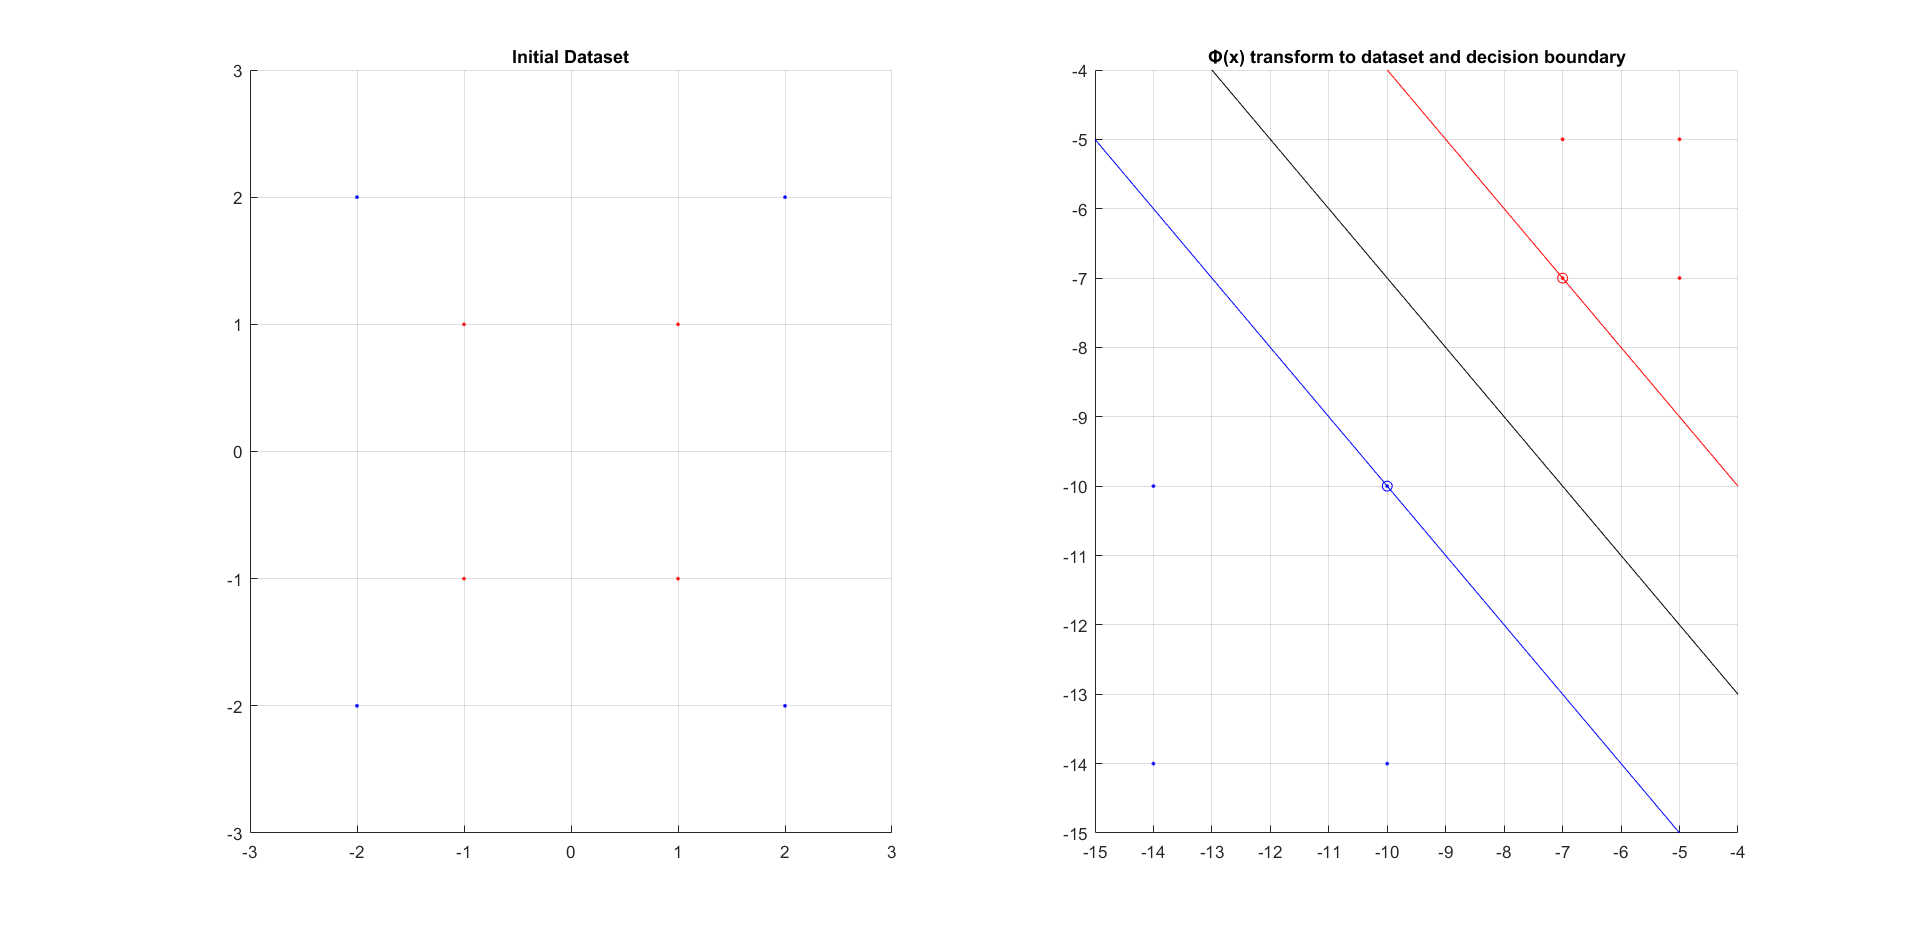
\includegraphics[height=6cm,width=\linewidth]{../exercise2_5/images/ex5_not_linear.png}
		\caption{Not Linear SVM}
	\end{figure}
	\noindent
	Όπως φαίνεται και στο πραπάνω διάγραμμα τα αρχικά δείγματα δεν είναι γραμμικώς διαχωρίσιμα, καθώς τα δείγματα της δεύτερης κλάσης βρίσκονται ανάμεσα στα δείγματα της κλάσης 1.
	
	\noindent 
	Για το λόγο αυτό θα εφαρμόσουμε τον παρακάτω γραμμικό μετασχηματισμό για να γίνουν διαχωρίσιμα τα δείγματα της κάθε κλάσης.
	\begin{align*}
		Φ(\vec{x}) = \vec{x} - \norm{\vec{x}}^2 - 4
	\end{align*}
	\noindent
	όπου το τετράγωνο της νόρμας των δειγμάτων της κλάσης 1 είναι ίση με $2^2 + 2^2 = 8$, ενώ της κλάσης 2 είναι $1^2 + 1^2 = 2$ 
	\noindent
	Οπότε τα μετασχημετισμένα δείγματα που προκύπτουν είναι 
	\begin{align*}
		ω_{1}: x^{+} = \{ [-10,-10]^{T}, [-10,-14]^{T}, [-14,-14]^{T}, [-14,-10]^{T} \} \\
		ω_{2}: x^{-} = \{ [-5,-5]^{T}, [-5,-7]^{T}, [-7,-7]^{T}, [-7,-5]^{T} \}
	\end{align*}
	\noindent
	Με βάση το παραπάνω διάγραμμα απεικόνισης το δειγμάτων, τα νέα support vectors είναι τα εξής:
	\begin{align*}
		S_{1} = [-10,-10]^{T}, \tab S_{2} = [-7,-7]^{T}
	\end{align*}
	Επιπλέον, η γραμμή διαχωρισμού θα είναι η μεσοκάθετος του ευθύγραμμου τμήματος που ενώνει τα δύο support vectors. Η κλίση αυτής της μεσοκαθέτου θα είναι -1, καθώς είναι κάθετη στο ευθύγραμμο τμήμα που ενώνει τα σημεία και η εξίσωση της ευθείας που διέρχεται από τα 2 support vectors έχει κλίση 1. Όσον αφορά το offset, βλέπουμε ότι διέρχεται από το σημείο (-13,-4). Άρα, το έχουμε offset ίσο με $-4 = -1 \cdot (-13) + β \Rightarrow β = -17 $. Συνεπώς, η ευθεία διαχωρισμού είναι η $y = -x - 17 $.\\
	
	\noindent
	Για τον αναλυτικό υπολογισμό της εξίσωσης διαχωρισμού θα χρησιμοποιήσουμε πολλαπλασιαστές Lagrange και τις συνθήκες Karush-Khun-Tucker (KKT). Επιπλέον, η συνάρτηση την οποία ελαχιστοποιούμε, καθώς και οι συνθήκες κάτω από τις οποίες γίνεται η ελαχιστοποίηση είναι ίδιες με την προηγούμενη περίπτωση όπου τα δείγματα ήταν γραμμικά διαχωρίσιμα.\\
	
	\begin{align*}
		S_{1} &= [-10,-10]^{T} : \ \ \ 1 \cdot ( -10 \cdot w_{1} + (-10) \cdot w_{2} + b) \ge 1 \Rightarrow 
		-10 \cdot w_{1} - 10 w_{2}  + b - 1 \ge 0 \\
		S_{2} &= [-7,-7]^{T} : \ \ \ -1 \cdot ( -7 \cdot w_{1} + (-7) \cdot w_{2} + b) \ge 1 \Rightarrow 
		7 \cdot w_{1} 7\cdot w_{2} - b - 1 \ge 0 \\
	\end{align*}	
	Από τις παραπάνω δυο σχέσεις βλέπουμε ότι οι ευθείες $-10 \cdot w_{1} - 10 w_{2}  + b - 1 = 0$ και $-7 \cdot w_{1} - 7\cdot w_{2} - b - 1 = 0 $ έχουν την ίδια κλίση αλλά διαφρετικά offsets. Επομἐνως, για να έχουμε 1 εξίσωση και για να μειώσουμε το χώρο αναζήτησης θα επίλέξουμε b τέτοιο ώστε να ισχύει το εξής
	\begin{align*}
		\frac{b - 1}{10} &= \frac{ -b - 1}{-7} \\
		(-7) \cdot (b - 1) &= 10 \cdot ( -b - 1) \\
		-7 \cdot b + 7 &= -10 \cdot b - 10 \\
		3 \cdot b = -17 \\
		b &= -\frac{17}{3}
	\end{align*}
	\noindent
	Eπομένως, τα υπερεπίπεδα διαχωρισμού γίνονται
	\begin{align*}
		S_{1} &= [-10,-10]^{T} : \ \ \ -10 \cdot w_{1} - 10 w_{2} - \frac{17}{3} - 1 \ge 0 \Rightarrow -10 \cdot w_{1} - 10 w_{2} - \frac{20}{3} \ge 0\\
		S_{2} &= [-7,-7]^{T} : \ \ \ 7 \cdot w_{1} + 7\cdot w_{2} - \left( -\frac{17}{3} \right) - 1 \ge 0 \Rightarrow 7 \cdot w_{1} + 7\cdot w_{2} + \frac{14}{3} \ge 0 \\
	\end{align*}

	\begin{align*}
		\mathcal{L}(w,b,λ_{1},λ_{2},λ_{3}) = \frac{1}{2} \cdot (w_{1}^{2} + w_{2}^{2}) - 
		λ_{1} \cdot \left(-10 \cdot w_{1} - 10 w_{2} - \frac{20}{3}\right) -
		λ_{2} \cdot \left(7 \cdot w_{1} + 7\cdot w_{2} + \frac{14}{3}\right)
	\end{align*}
	
	\noindent
	Οι συνθήκες KKT είναι οι εξής:\\
	
	\noindent
	(1) $\Rightarrow$
	\begin{align*}
		\frac{\partial \mathcal{L}(w,b,λ_{1},λ_{2},λ_{3})}{\partial w_{1}} &= w_{1} + 10 \cdot λ_{1} - 7 \cdot λ_{2} = 0 \\
		\frac{\partial \mathcal{L}(w,b,λ_{1},λ_{2},λ_{3})}{\partial w_{2}} &= w_{2} + 10 \cdot λ_{1} - 7 \cdot λ_{2} = 0 \\
		\frac{\partial \mathcal{L}(w,b,λ_{1},λ_{2},λ_{3})}{\partial b} &= - λ_{1} + λ_{2} = 0
	\end{align*}
	\noindent
	(2) $\Rightarrow$
	\begin{align*}
		λ_{1} \cdot \left(-10 \cdot w_{1} - 10 w_{2} - \frac{20}{3}\right) &= 0 \\
		λ_{2} \cdot \left(7 \cdot w_{1} + 7 \cdot w_{2} + \frac{14}{3}\right) &= 0
	\end{align*}	
	\noindent
	(3) $\Rightarrow$
	\begin{align*}
		-10 \cdot w_{1} - 10 \cdot w_{2} - \frac{20}{3} \ge 0 \\
		7 \cdot w_{1} + 7\cdot w_{2} + \frac{14}{3} \ge 0 
	\end{align*}
	\noindent
	(4) $\Rightarrow$
	\begin{align*}
		λ_{i} \ge 0, \tab \forall i = 1, 2, 3
	\end{align*}	
	\noindent
	Διακρίνουμε τις παρακάτω 4 περιπτώσεις ανάλογα με την τιμή του κάθε $λ_{i}$\\
	
	\noindent
	1) Αν $λ_{1} = 0$, $λ_{2} = 0$	\\
	Τότε από τις σχέσεις (1) έχουμε
	\begin{align*}
		w_{1} + 10 \cdot 0 - 7 \cdot 0 = 0 \Rightarrow w_{1} = 0 \\
		w_{2} + 10 \cdot 0 - 7 \cdot 0 = 0 \Rightarrow w_{2} = 0 \\
	\end{align*}
	\noindent
	Από τις σχέσεις (3) έχουμε 
	\begin{align*}
		-10 \cdot 0 - 10 \cdot 0 - \frac{20}{3} \ge 0 \Rightarrow - \frac{20}{3} \ge 0 \tab \textit{Άτοπο} \\
		7 \cdot 0 + 7\cdot 0 + \frac{14}{3} \ge 0 \Rightarrow \frac{14}{3} \ge 0 \tab \textit{Ισχύει}
	\end{align*}
	\noindent
	Συνεπώς, επειδή οι παραπάνω σχέσεις δεν επαληθεύονται όλες, οι αρχική υπόθεση για τα λ δεν ισχύει.\\
	
	\noindent
	2) Αν $λ_{1} = 0$, $λ_{2} \ne 0$	\\
	Τότε από τις σχέσεις (1) έχουμε
		\begin{align*}
		w_{1} + 10 \cdot 0 - 7 \cdot λ_{2} = 0 \Rightarrow w_{1} = 7 \cdot λ_{2} \\
		w_{2} + 10 \cdot 0 - 7 \cdot λ_{2} = 0 \Rightarrow w_{2} = 7 \cdot λ_{2} \\
	\end{align*}
	\noindent
	Eπιπλέον, από τις σχέσεις (2) και εφόσον $λ_{2} \ne 0 $ προκύπτει
	\begin{align*}
		7 \cdot w_{1} + 7 \cdot w_{2} + \frac{14}{3} = 0 \Rightarrow 7 \cdot 7 \cdot λ_{2} + 7 \cdot  7 \cdot λ_{2} + \frac{14}{3} = 0 \Rightarrow λ_{2} = - \frac{14}{294} 
	\end{align*}
	\noindent
	Η τιμή $λ_{2} = - \frac{14}{294} $ έρχεται σε αντίθεση με την 4η συνθήκη ΚΚΤ όπου πρέπει το κάθε λ να είναι μεγαλύτερο ή ίσο με το 0.\\
	
	\noindent
	3) Αν $λ_{1} \ne 0$, $λ_{2} = 0$ \\
	Τότε από τις σχέσεις (1) έχουμε
	\begin{align*}
		w_{1} + 10 \cdot λ_{1} - 7 \cdot 0 = 0 \Rightarrow w_{1} = -10 \cdot λ_{1} \\
		w_{2} + 10 \cdot λ_{1} - 7 \cdot 0 = 0 \Rightarrow w_{2} = -10 \cdot λ_{1} \\
		λ_{1} = λ_{2}
	\end{align*}
	\noindent
	Eπιπλέον, από τις σχέσεις (2) και εφόσον $λ_{1} \ne 0 $ προκύπτει
	\begin{align*}
		-10 \cdot w_{1} - 10 \cdot w_{2} + \frac{20}{3} = 0 \Rightarrow 10 \cdot (-10) \cdot λ_{1} -10 \cdot (-10) \cdot λ_{1} + \frac{20}{3} = 0 \Rightarrow λ_{1} = \frac{1}{30} 
	\end{align*}
	\noindent
	Αντικαθιστώντας στις παραπάνω σχέσεις προκύπτουν
	\begin{align*}
		w_{1} = -10 \cdot λ_{1} \Rightarrow w_{1} = -10 \cdot \frac{1}{30} = -\frac{1}{3} \\
		w_{2} = -10 \cdot λ_{1} \Rightarrow w_{2} = -10 \cdot \frac{1}{30} = -\frac{1}{3} \\
	\end{align*}
	\noindent
	Τέλος, αντικαθιστώντας στις σχέσεις (3) έχουμε
	\begin{align*}
		-10 \cdot \left(-\frac{1}{3}\right) - 10 \cdot \left(-\frac{1}{3}\right) - \frac{20}{3} \ge 0 \Rightarrow 0 \ge 0 \tab \textit{Ισχύει}\\
		7 \cdot \left(-\frac{1}{3}\right) + 7\cdot \left(-\frac{1}{3}\right) + \frac{14}{3} \ge 0 \tab \textit{Ισχύει} 
	\end{align*}
	\noindent
	Ωστόσο, από τις σχέσεις (1) προκύπτει ότι το $λ_{1} = λ_{2}$ το οποίο έρχεται σε αντίθεση με την αρχική υπόθεση.
	
	\noindent
	4) Αν $λ_{1} \ne 0$, $λ_{2} \ne 0$ \\
	Τότε από τις σχέσεις (1) έχουμε
	\begin{align*}
		λ_{1} &= λ_{2} \\
		w_{1} + 10 \cdot λ_{1} - 7 \cdot λ_{2} &= 0 \Rightarrow w_{1} = -10 \cdot λ_{1} + 7 \cdot λ_{1} \Rightarrow  w_{1} = -3 \cdot λ_{1}\\
		w_{2} + 10 \cdot λ_{1} - 7 \cdot λ_{2} &= 0 \Rightarrow w_{2} = -10 \cdot λ_{1} + 7 \cdot λ_{1} \Rightarrow  w_{2} = -3 \cdot λ_{1}\\
	\end{align*}
	Επιπλέον, από τις σχέσεις (2) και εφόσον τα λ είναι διαφορετικά το 0 προκύπτει
	\begin{align*}
		-10 \cdot w_{1} - 10 \cdot w_{2} - \frac{20}{3} &= 0 \Rightarrow -10 \cdot (-3 \cdot λ_{1}) - 10 \cdot (-3 \cdot λ_{1}) - \frac{20}{3} = 0 \Rightarrow 60 \cdot λ_{1} = \frac{20}{3} \Rightarrow λ_{1} = \frac{1}{9}\\
	\end{align*}
	\noindent
	Αντικαθιστώντας την τιμή του $λ_{1}$ προκύπτει ότι
	\begin{align*}
		w_{1} = -3 \cdot λ_{1} \Rightarrow w_{1} = -3 \cdot \frac{1}{9} = -\frac{1}{3}\\
		w_{2} = -3 \cdot λ_{1} \Rightarrow w_{2} = -3 \cdot \frac{1}{9} = -\frac{1}{3}
	\end{align*}
	\noindent
	Από τις σχέσεις (3) ελέγχουμε αν είμαστε εντός feasible region
	\begin{align*}
		-10 \cdot \left( -\frac{1}{3} \right) - 10 \cdot \left( -\frac{1}{3} \right) - \frac{20}{3} \ge 0 \Rightarrow 0 \ge 0 \tab \textit{Ισχύει}\\
		7 \cdot \left( -\frac{1}{3} \right) + 7 \cdot \left( -\frac{1}{3} \right) + \frac{14}{3} \ge 0 \Rightarrow 0 \ge 0 \tab \textit{Ισχύει}
	\end{align*}
	
	\noindent
	Συνεπώς, η ευθεία που προκύπτει είναι η εξής
	\begin{align*}
		w^{T} \cdot \vec{x} + b &= 0 \Rightarrow \\
		\begin{bmatrix}
			-\frac{1}{3} \\
			-\frac{1}{3}
		\end{bmatrix} \cdot 
		\begin{bmatrix}
			x & y 
		\end{bmatrix} + \left(-\frac{17}{3}\right) &= 0 \Rightarrow \\
		-\frac{1}{3}  \cdot x - \frac{1}{3} \cdot y -\frac{17}{3} &= 0 \Rightarrow\\
		 x + y + 17 &= 0 \Rightarrow
		 y = -x - 17
	\end{align*}

\pagebreak
\section*{Άσκηση 6: Support Vector Machines (Εφαρμογή σε τεχνητό σύνολο δεδομένων)}
	Έστω ότι έχουμε ένα σύνολο δειγμάτων $\{ (x^{(1)}, y^{(1)}), (x^{(2)}, y^{(2)}), \cdots , (x^{(n)}, y^{(n)}) \}$, όπου $x^{(i)} \in \mathbb{R}^{1 \times 2 }$ και $y^{(i)} \in \{-1,1\}$. Σκοπός της άσκησης είναι να προβλέψουμε τις τιμές  $y^{(i)}$ από τις αντίστοιχες $x^{(i)}$ χρησιμοποιώντας Support Vector Machines (SVM).\\
	
	\noindent
	Η Λαγκρανζιανή του δυικού προβλήματος είναι η παρακάτω
	\begin{align*}
		\mathcal{L}(λ) &= \sum_{i=1}^{n} λ_{i} - 
							\frac{1}{2} \cdot \sum_{i=1}^{n} \sum_{j=1}^{n} λ^{(i)} \cdot λ^{(j)} \cdot y^{(i)} \cdot y^{(j)} \cdot x^{(i)} \cdot (x^{(j)})^T \\
					  &= 
					  \begin{bmatrix}
					  	1 \\
					  	\vdots \\
					    1
					  \end{bmatrix}^{T} \cdot 
					  \begin{bmatrix}
					     λ_{1} \\
						 \vdots \\
						 λ_{n}
					  \end{bmatrix} - 
					  \frac{1}{2} \cdot 
					  \begin{bmatrix}
							  	λ_{1} \\
							  	\vdots \\
							  	λ_{n}
					  \end{bmatrix}^{T} \cdot H \cdot
					  \begin{bmatrix}
							  	λ_{1} \\
							  	\vdots \\
							  	λ_{n}
					  \end{bmatrix}
	\end{align*}
	\noindent
	όπου $Η = y^{(i)} \cdot y^{(j)} \cdot x^{(i)} \cdot (x^{(j)})^T$  και επιπλέον μεγιστοποιούμε την παραπάνω Λαγκρανζιανή υπό τους παρακάτω περιορισμούς
	\begin{align*}
		λ^{(i)} \ge 0, \tab i=1,2, \cdots, n \\
		\sum_{i=1}^{n} λ^{(i)} \cdot y^{(i)} = 0
	\end{align*}	
	\noindent
	Ωστόσο, η συνάρτηση quadprog() που θα χρησιμοποιήσουμε ελαχιστοποιεί την παρακάτω σχέση
	\begin{align*}
		f^{T} \cdot x + \frac{1}{2} \cdot x^{T} \cdot H \cdot x \ \ \ \textit{έτσι ώστε} \ \ \
		\begin{cases}
			A \cdot x \le b,\\
			A_{eq} \cdot x = b_{eq}, \\
			l_{b} \le x \le u_{b}
		\end{cases}
	\end{align*}
	\noindent
	Αν πολλαπλασιάσουμε τη Λαγκρανζιανή με -1 τότε προκύπτει
	\begin{align*}
		\mathcal{L}(λ) &= 
		\begin{bmatrix}
			-1 \\
			\vdots \\
			-1
		\end{bmatrix}^{T} \cdot 
		\begin{bmatrix}
			λ_{1} \\
			\vdots \\
			λ_{n}
		\end{bmatrix} + 
		\frac{1}{2} \cdot 
		\begin{bmatrix}
			λ_{1} \\
			\vdots \\
			λ_{n}
		\end{bmatrix}^{T} \cdot H \cdot
		\begin{bmatrix}
			λ_{1} \\
			\vdots \\
			λ_{n}
		\end{bmatrix}
	\end{align*}
 	\noindent
 	Έτσι προκύπτουν οι πίνακες f και H που θα χρησιμοποιηθούν ως ορίσματα στη συνάρτηση quadprog. Όσον αφορά τα υπόλοιπα ορίσματα για το vectors Α και b χρησιμοποιούμε ένα κενό vector, καθώς ο συγκεκριμένος περιορισμός δεν μας χρειάζεται. Επιπλέον, ο πίνακας $A_{eq}$ θα είναι ο $y^T$, ενώ το $b_{eq}$ το θέλουμε να είναι ίσο με 0, για να ικανοποιείται ο δεύτερος περιορισμός. Τέλος, για τον πρώτο περιορισμό θέλουμε το vector $l_{b}$ να είναι ένα vector αρχικοποιημένο με μηδενικά, ενώ το vector $u_{b}$ το αρχικοποικούμε με την τιμή Inf (άπειρο), εφόσον θέλουμε το κάθε $λ^{(i)} \ge 0$. \\ 
 	
 	\noindent
 	Έπειτα, από τον υπολογισμό των λ, βρίσκουμε το w, $w_{0}$  και το width of margin με βάση τους παρακάτω τύπους
 	\begin{align*}
 		w &= \sum_{i=1}^{n} λ^{(i)} \cdot y_{(i)} \cdot x_{(i)}\\
 		w_{0} &= \frac{1}{m} \cdot \sum_{i=1}^{m}(y_{i} - x_{i} \cdot w)\\
 		d &= - \frac{w_{0}}{max\{ \norm{w}\}}
 	\end{align*}
 
 	\pagebreak
	\noindent
	Τα αποτελέσματα που προκύπτουν από την εκτέλεση του αλγορίθμου είναι τα εξής
	\begin{figure}[h!]
		\centering
		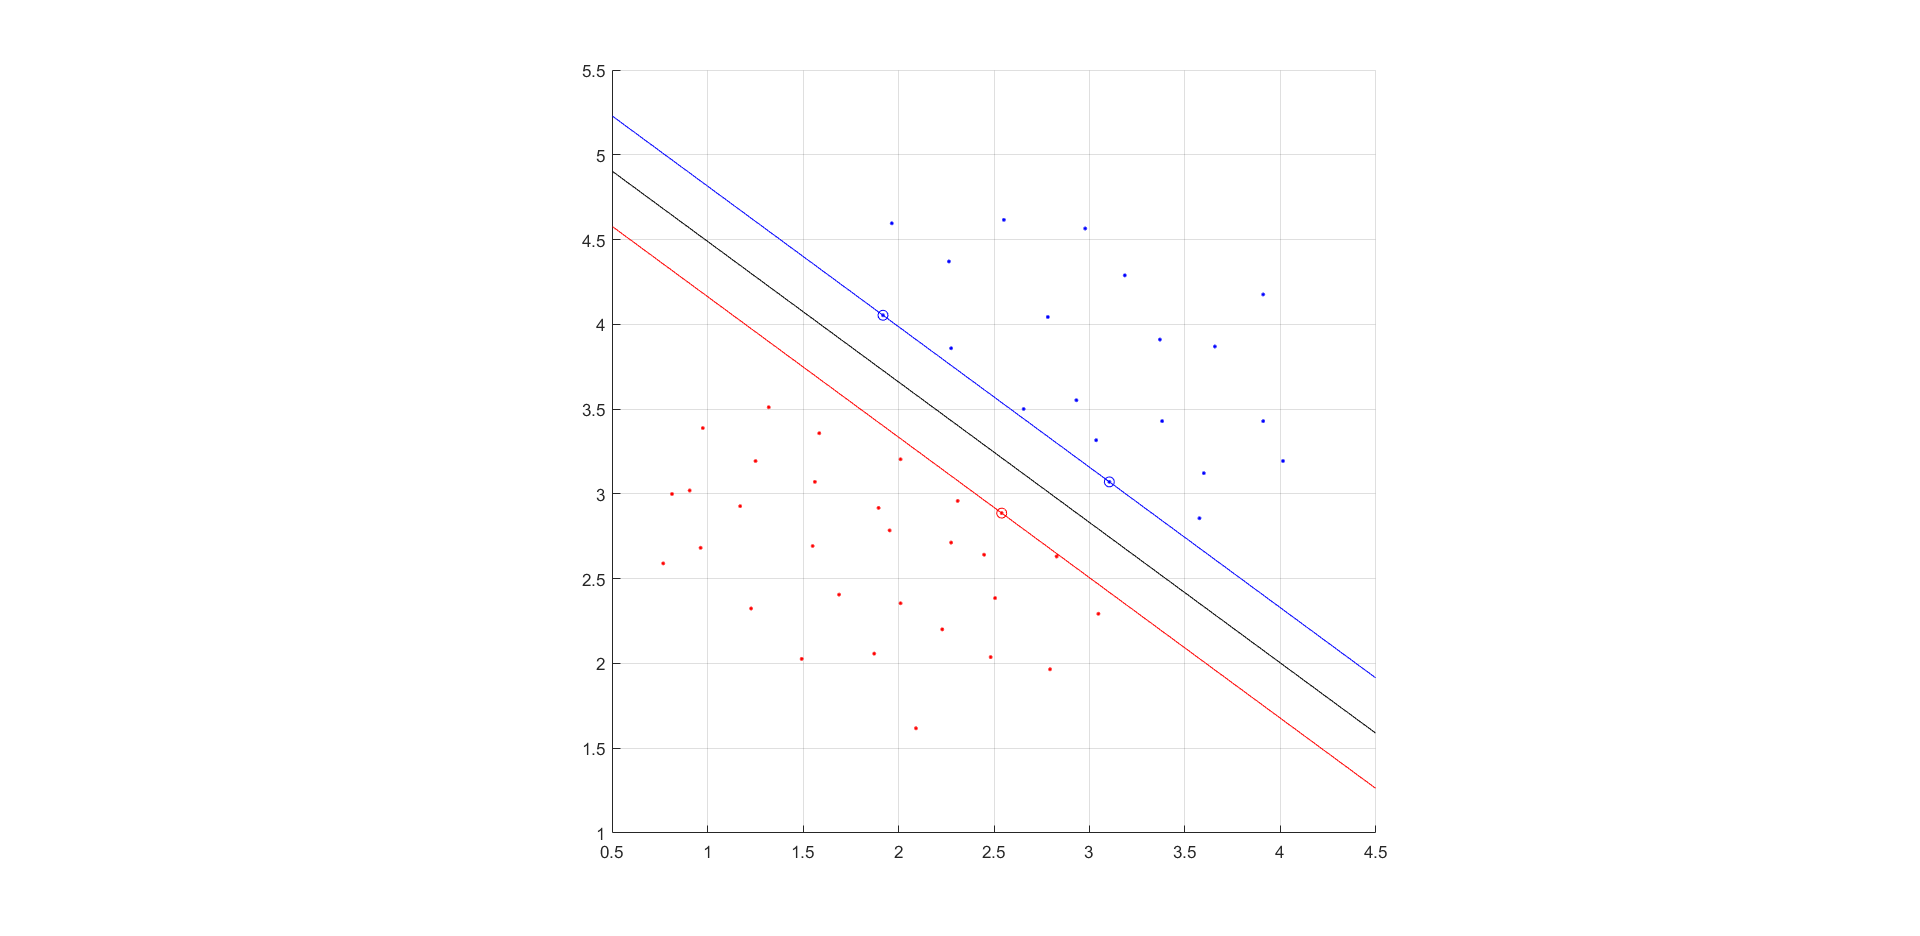
\includegraphics[height=6cm,width=\linewidth]{../exercise2_6/images/ex6_ex1_C_100.png}
		\caption{SVM using only 50 out of 51 samples}
	\end{figure}

	\noindent
	Για το δεύτερο μέρος της άσκησης θα χρησιμοποιήσουμε και τα 51 δείγματα του αρχείου και θα γίνει χρήση κάποιων slack variables, τα οποία χρησιμοποιούνται όταν υπάρχει θόρυβος στα δεδομένα έτσι ώστε να γίνονται ανεκτά κάποια δείγματα στη λάθος πλευρά της επιφάνειας απόφασης. Η Λαγκρανζιανή που θα χρησιμοποιήσουμε είναι ίδια με του προηγούμενου ερωτήματος. Ωστόσο, προστίθεται ακόμα η εξής συνθήκη
	 \begin{align*}
		0 \le λ^{(i)} \le C, \tab i = 1, 2, \cdots, n
	\end{align*}
	\noindent
	Το μοναδικό πράγμα που αλλάζει από άποψη κώδικα είναι ότι αντί για την αρχικοποίηση σε Ιnf του vecotr $u_{b}$ το αρχικοποιούμε με C σε κάθε θέση του. Οπότε τα αποτελέσματα που προκύπτουν είναι τα εξής:

	\begin{figure}[h!]
		\centering
		\begin{subfigure}[t]{0.5\textwidth}
			\centering
			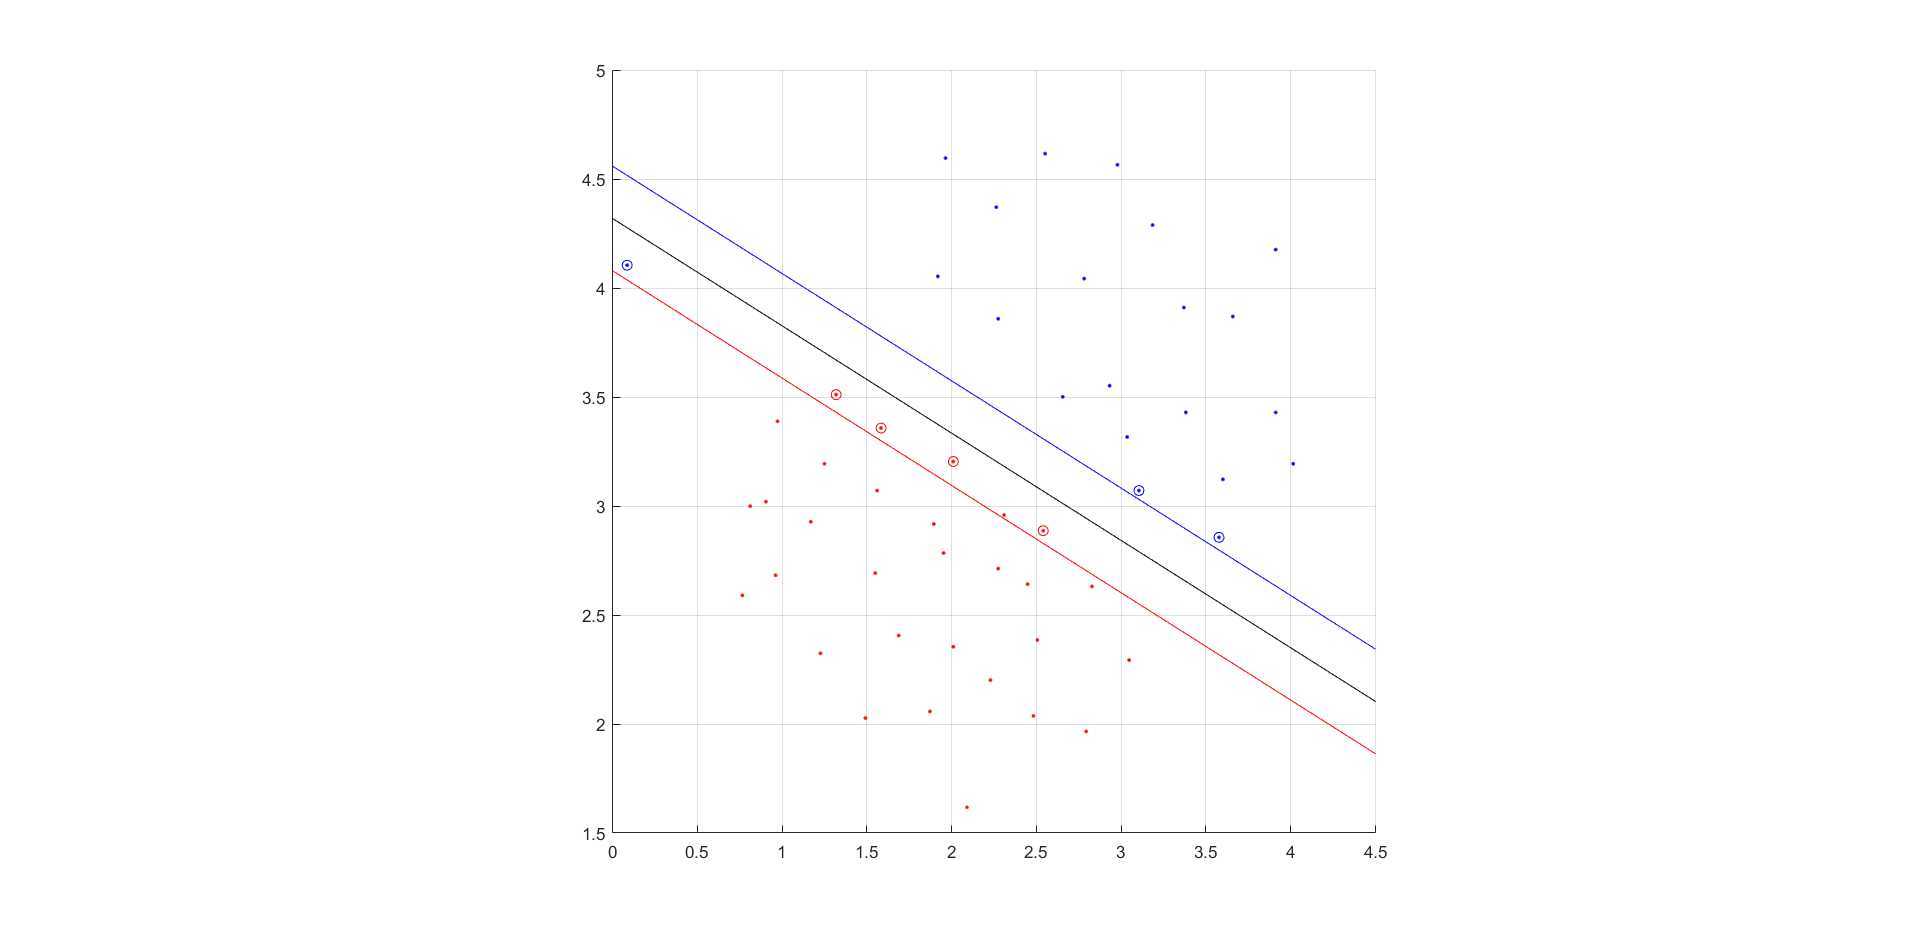
\includegraphics[height=5cm, width=\linewidth]{../exercise2_6/images/ex6_ex2_C_10.png}
			\caption{C = 10}
		\end{subfigure}%
		~
		\begin{subfigure}[t]{0.5\textwidth}
			\centering
			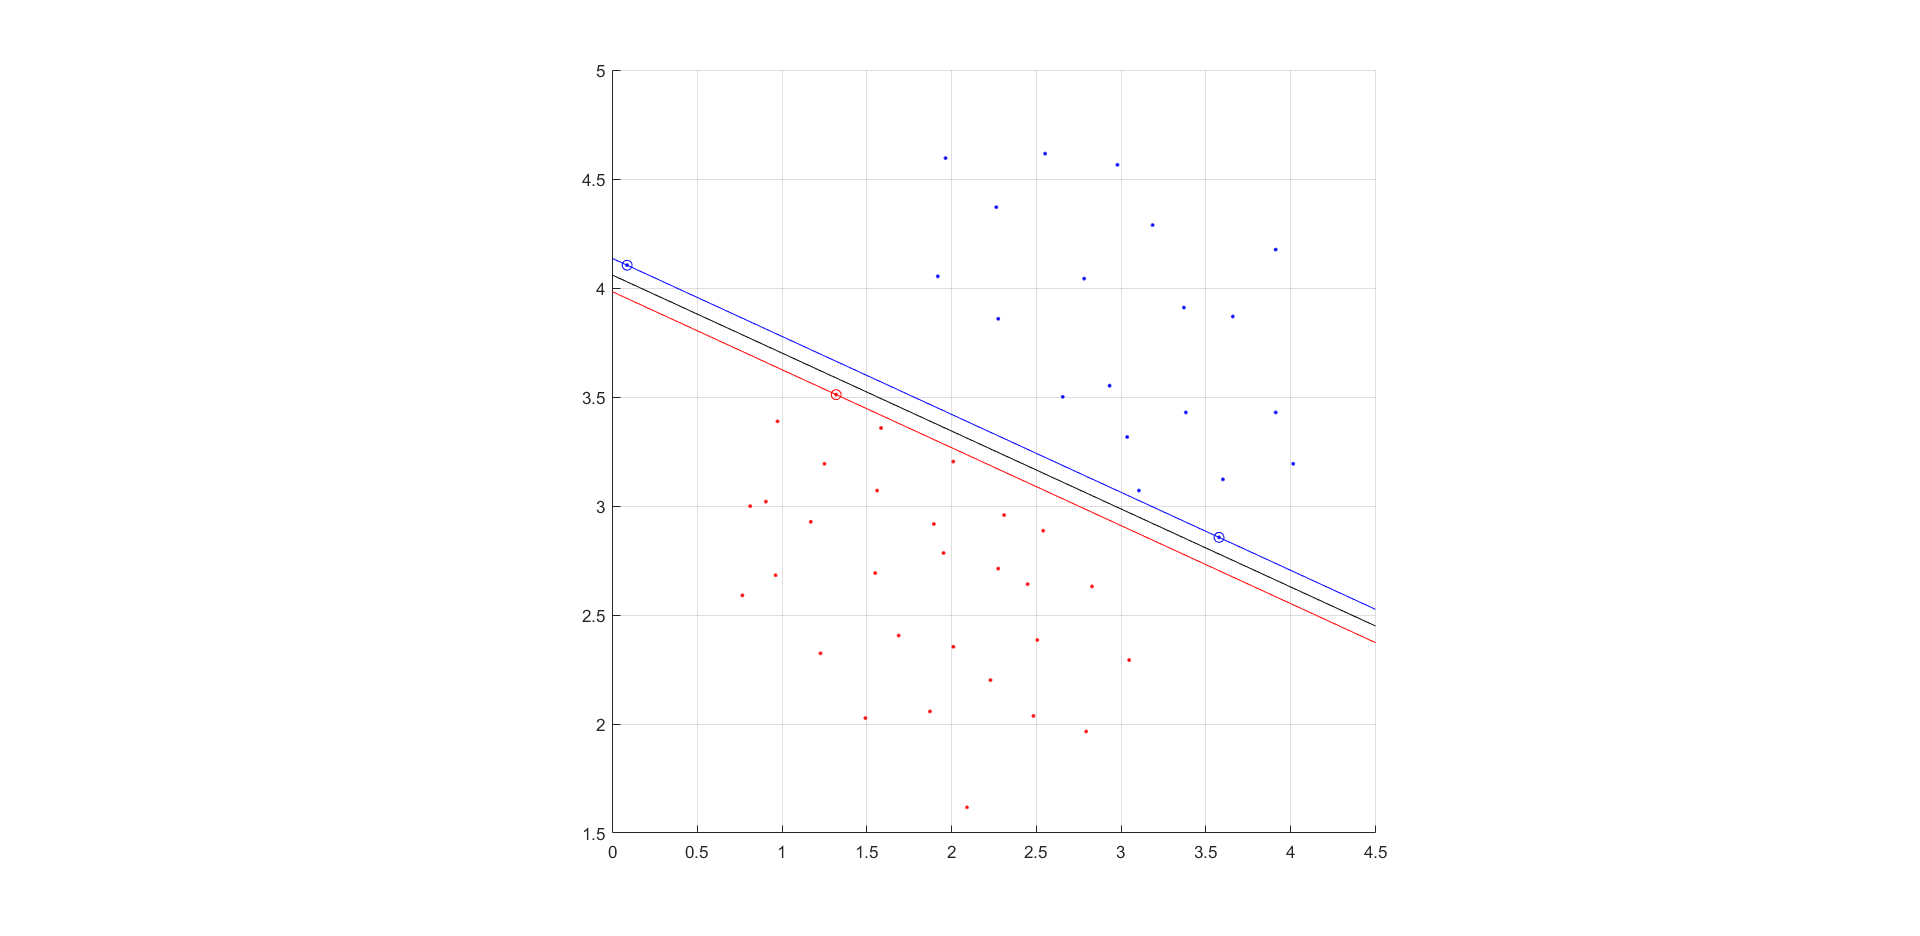
\includegraphics[height=5cm, width=\linewidth]{../exercise2_6/images/ex6_ex2_C_100.png}
			\caption{C = 100}
		\end{subfigure}
	\end{figure}
 	\noindent
 	Αυτό που παρατηρούμε είναι ότι όσο η τιμή της παραμέτρου C πλησιάζει στο 0 έχουμε μέγιστη ανοχή και κατ΄ επέκταση ενδέχεται κάποιο δείγμα που ανήκει πχ στην κλάση 1 να κατηγοριοποιηθεί στην κλάση 2, ενώ όσο αυξάνεται η τιμή του C έχουμε μηδενική ανοχή. 
 	
 	\noindent
 	Στο τρίτο και τελευταίο μέρος της άσκησης, θα χρησιμοποιήσουμε κάποια δείγματα τα οποία δεν είναι γραμμικώς διαχωρίσιμα με την ίδια Λαγκρανζιανή των προηγούμενων ερωτημάτων. Ακριβώς επειδή τα δείγματα δεν είναι γραμμικώς διαχωρίσιμα θα χρησιμοποιήσουμε ως τρίτο χαρακτηριστικό το τετράγωνο του μέτρου κάθε δείγματος. Γι'αυτό το λόγο θα προσθέσουμε μία τρίτη στήλη στον πίνακα Χ με αυτό το χαρακτηριστικό. Tα βήματα του αλγορίθμου για τον υπολογισμό των λ, w, $w_{0}$ και width of margin είναι ίδια με του προηγούμενου ερωτήματος. Τα αποτελέσματα που προέκυψαν είναι τα παρακάτω 
 	
 	\begin{figure}[h!]
 		\centering
 		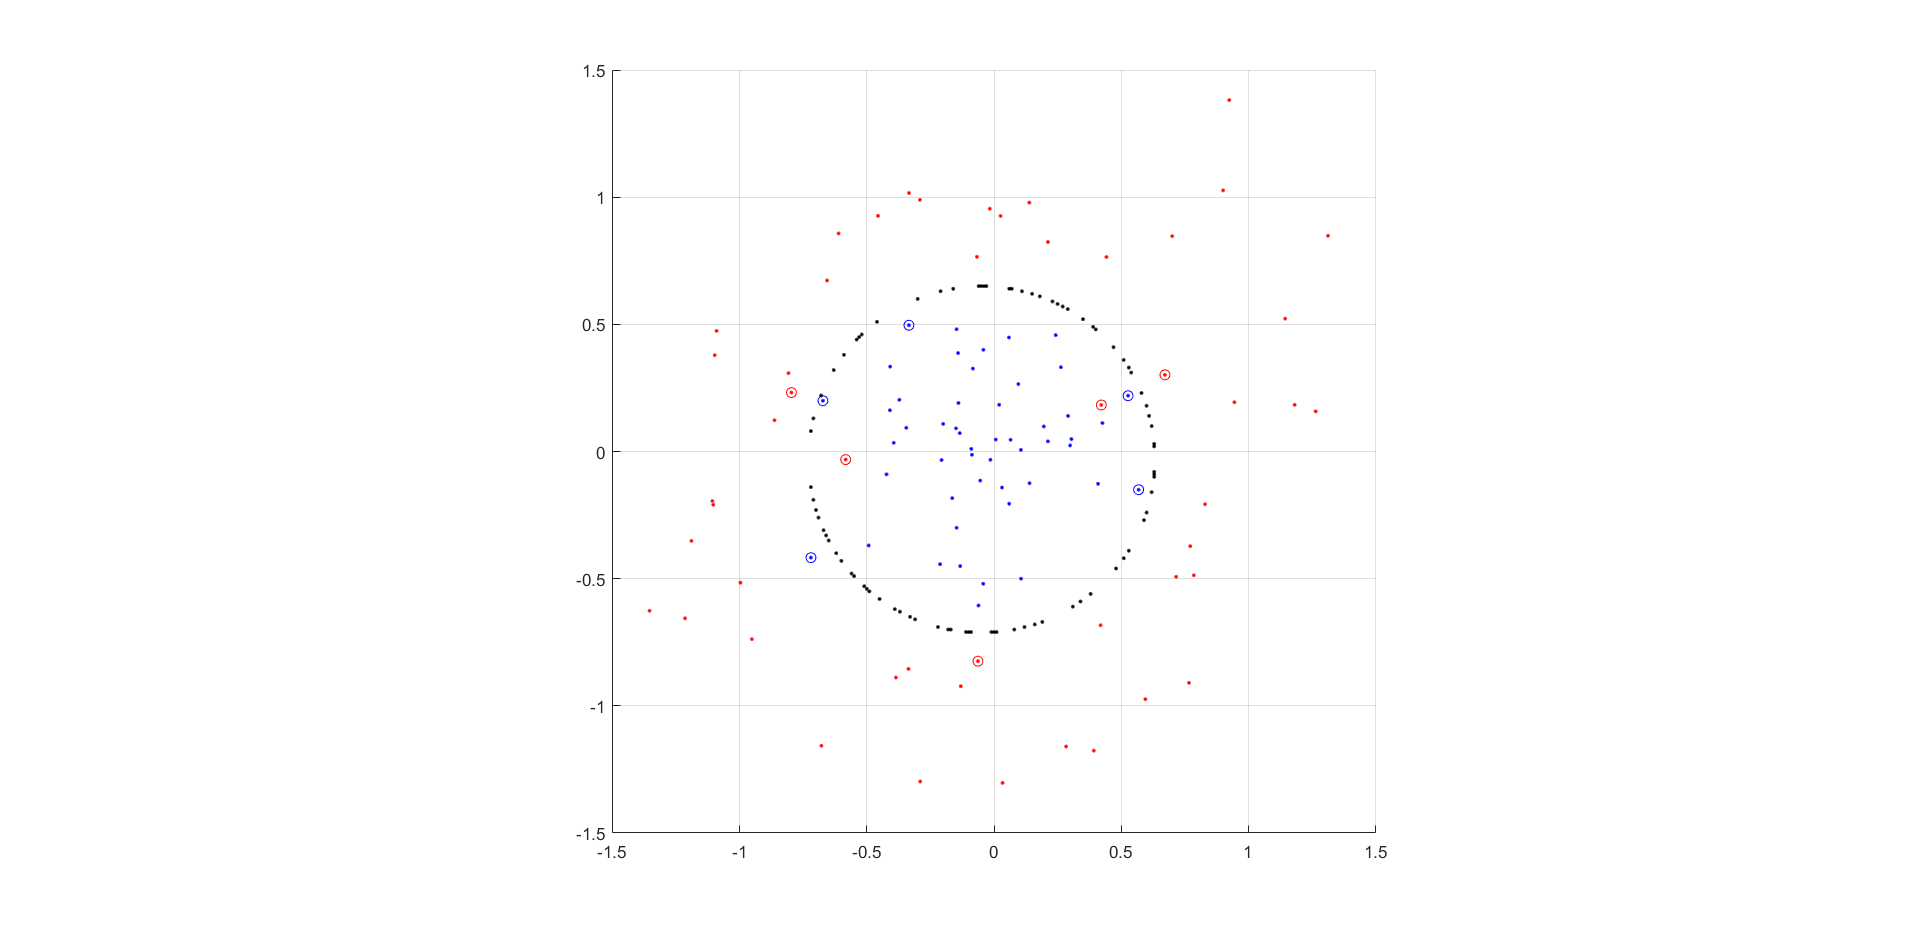
\includegraphics[height=6cm,width=\linewidth]{../exercise2_6/images/ex6_ex3_C_100.png}
 		\caption{SVM - Νot Linearly Separatable samples }
 	\end{figure}
 	\noindent
 	Από το παραπάνω διάγραμμα παρατηρούμε ότι προκύπτει ένα αρκετά ικανοποιητικό decision boundary. Ωστόσο, υπάρχουν κάποια ελάχιστα δείγματα της κόκκινης κλάσης (2 δείγματα) εντός της περιοχής απόφασης της μπλε κλάσης, ενώ συμβαίνει και το αντίθετο, δηλάδή υπάχει ένα μπλε δείγμα στην περιοχή απόφασης της κόκκινης κλάσης. 
\end{document}
